\section{Resultados}

En esta sección se describen los resultados empíricos del estudio, comenzando por las estadísticas descriptivas y la fiabilidad de los instrumentos, continuando con la validación factorial exploratoria y confirmatoria de la estructura de cinco factores, la depuración de ítems mediante Teoría de Respuesta al Ítem (TRI) y, finalmente, la prueba de las hipótesis mediante modelos de ecuaciones estructurales (SEM) completos y parsimoniosos.

\subsection{Descriptivos y fiabilidad}
Se analizaron las distribuciones de las cinco escalas a partir de las 452 respuestas válidas. La escala \emph{Skill--Job Fit} presentó una concentración notable de respuestas en los valores altos (5–7), con un 87,6\,\% de respuestas en ese rango; su moda fue 6 (39,7\,\%), la media por ítem osciló entre 5,56 y 5,80 y la media global fue $M=5{,}67$. La escala \emph{Personality--Job Fit} mostró resultados similares, con 90\,\% de respuestas en 5–7, media global $M=5{,}69$ y mediana 6, evidenciando un alto ajuste entre rasgos personales y el contexto laboral. Para el \emph{Apoyo Organizacional Percibido} (POS) el 83,6\,\% de las respuestas se concentró en 5–7, con media global $M=5{,}58$ y pico en 6 (33\,\%). La \emph{Satisfacción Laboral} presentó una distribución algo más dispersa: 75\,\% de respuestas en 5–7, moda en 5 (29,5\,\%) y media global $M=5{,}23$. Finalmente, la \emph{Intención de Renuncia} evidenció una clara asimetría negativa: 55\,\% de respuestas en 1–2, media $M=2{,}80$ y mediana 2. En conjunto, las escalas mostraron sesgos moderados (negativos en ajuste, POS y satisfacción; positivos en intención de renuncia), sin violaciones severas a la normalidad ordinal. Estos patrones sugieren un alto grado de ajuste persona–trabajo y satisfacción, un elevado apoyo percibido y una baja intención de renuncia.

Para mostrar visualmente estas distribuciones, la Figura \ref{fig:histogramas} presenta los histogramas de frecuencia de cada escala. Se observa que \emph{Skill}, \emph{Personality} y \emph{POS} se concentraron fuertemente en las categorías altas (sesgo negativo), mientras que \emph{Intention} se concentró en las categorías bajas (sesgo positivo) y \emph{Satisfaction} mostró una distribución algo más homogénea.

\begin{figure}[htbp]
\centering
\begin{tabular}{cc}
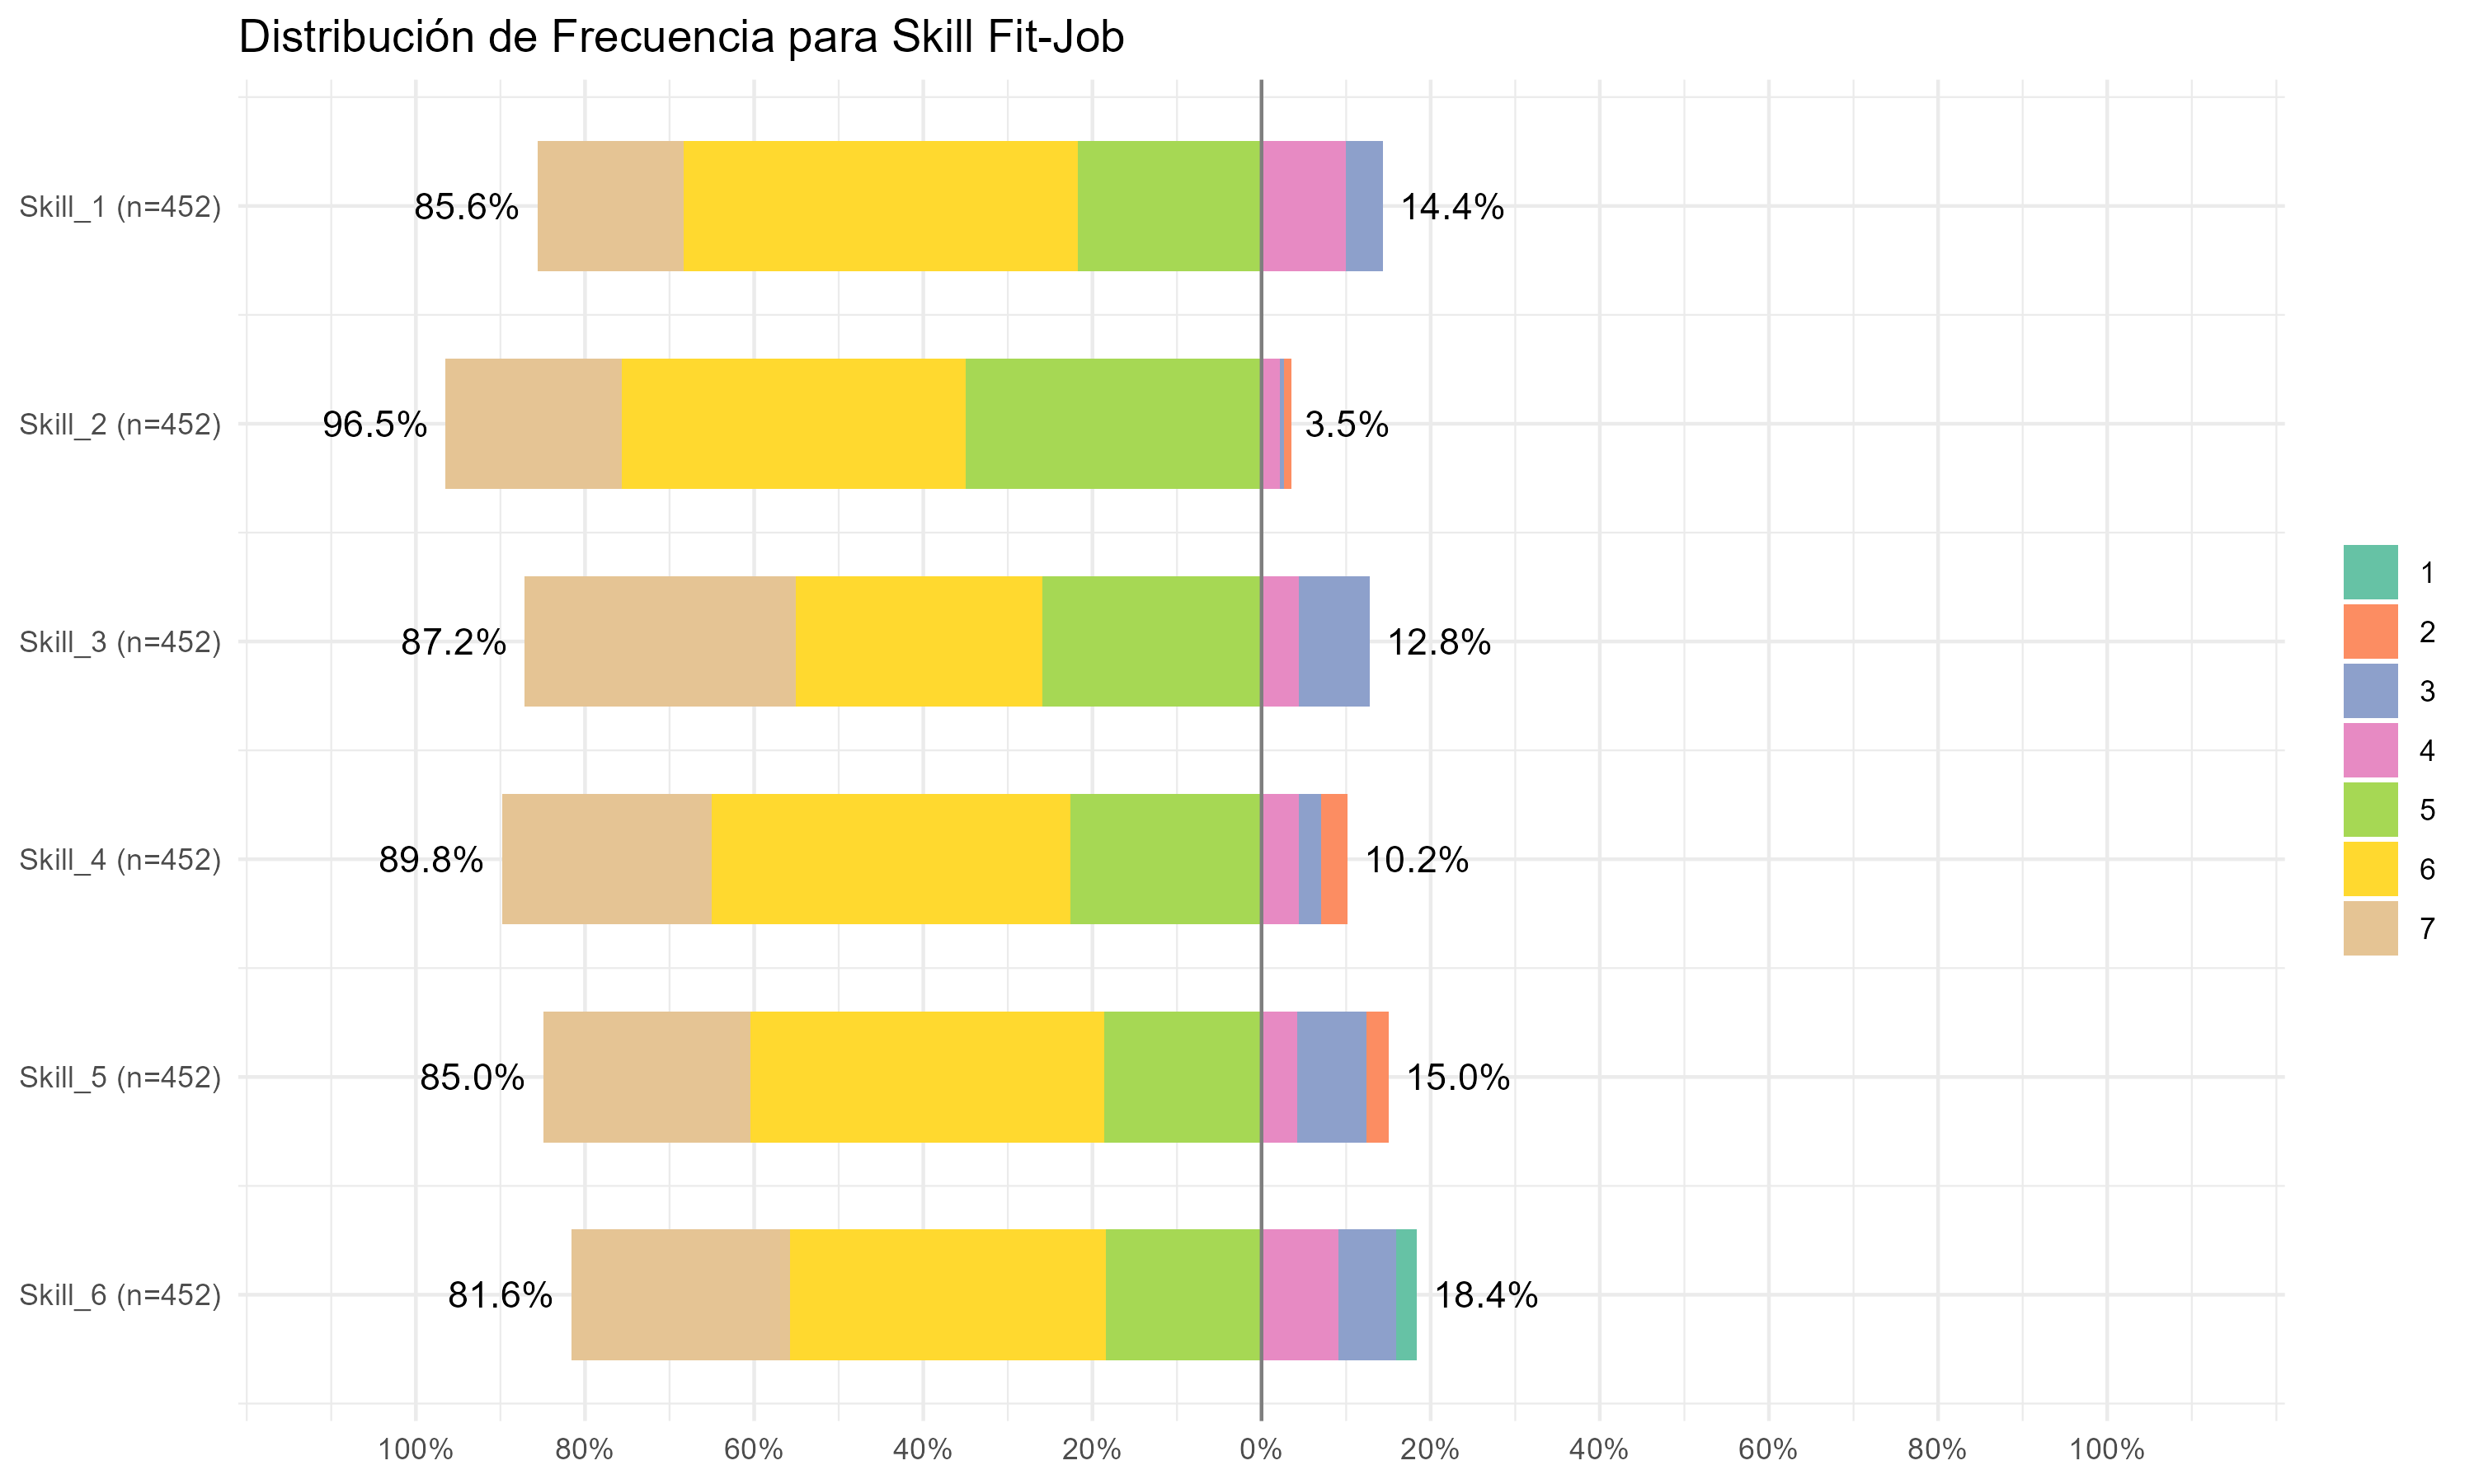
\includegraphics[width=0.45\textwidth]{figures/distribucion_frecuencia_skill.png} & 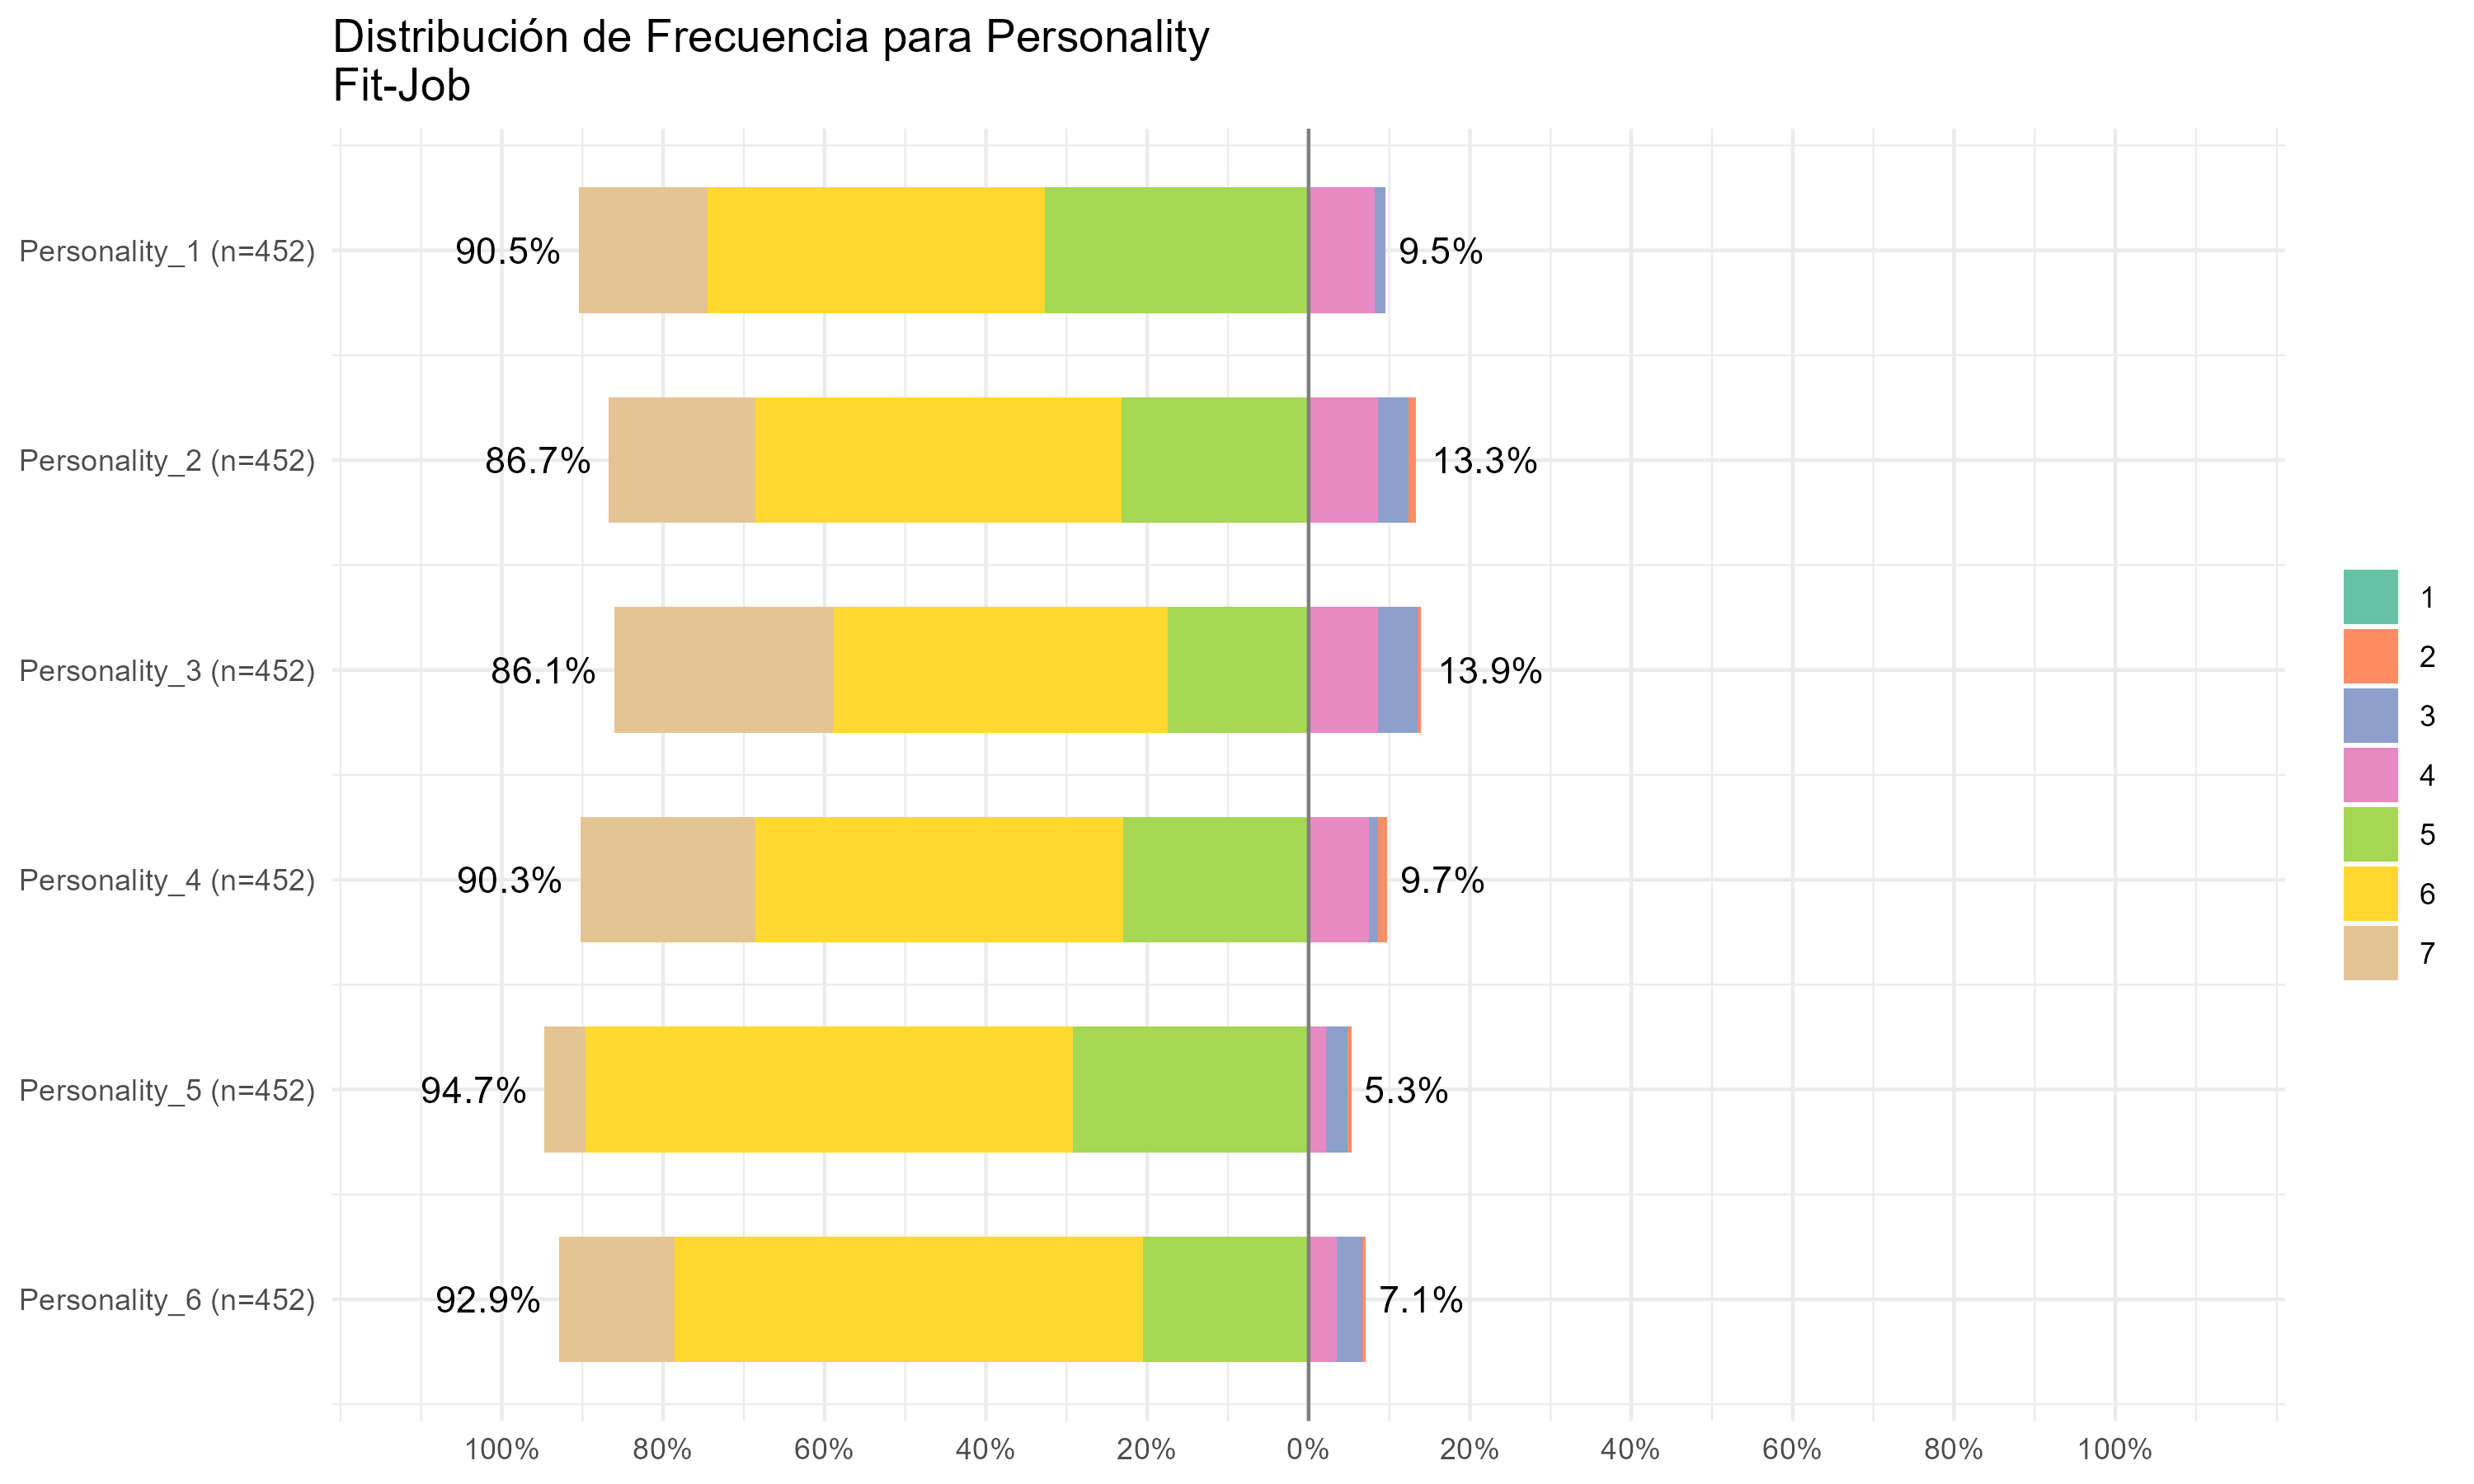
\includegraphics[width=0.45\textwidth]{figures/distribucion_frecuencia_personality.png} \\
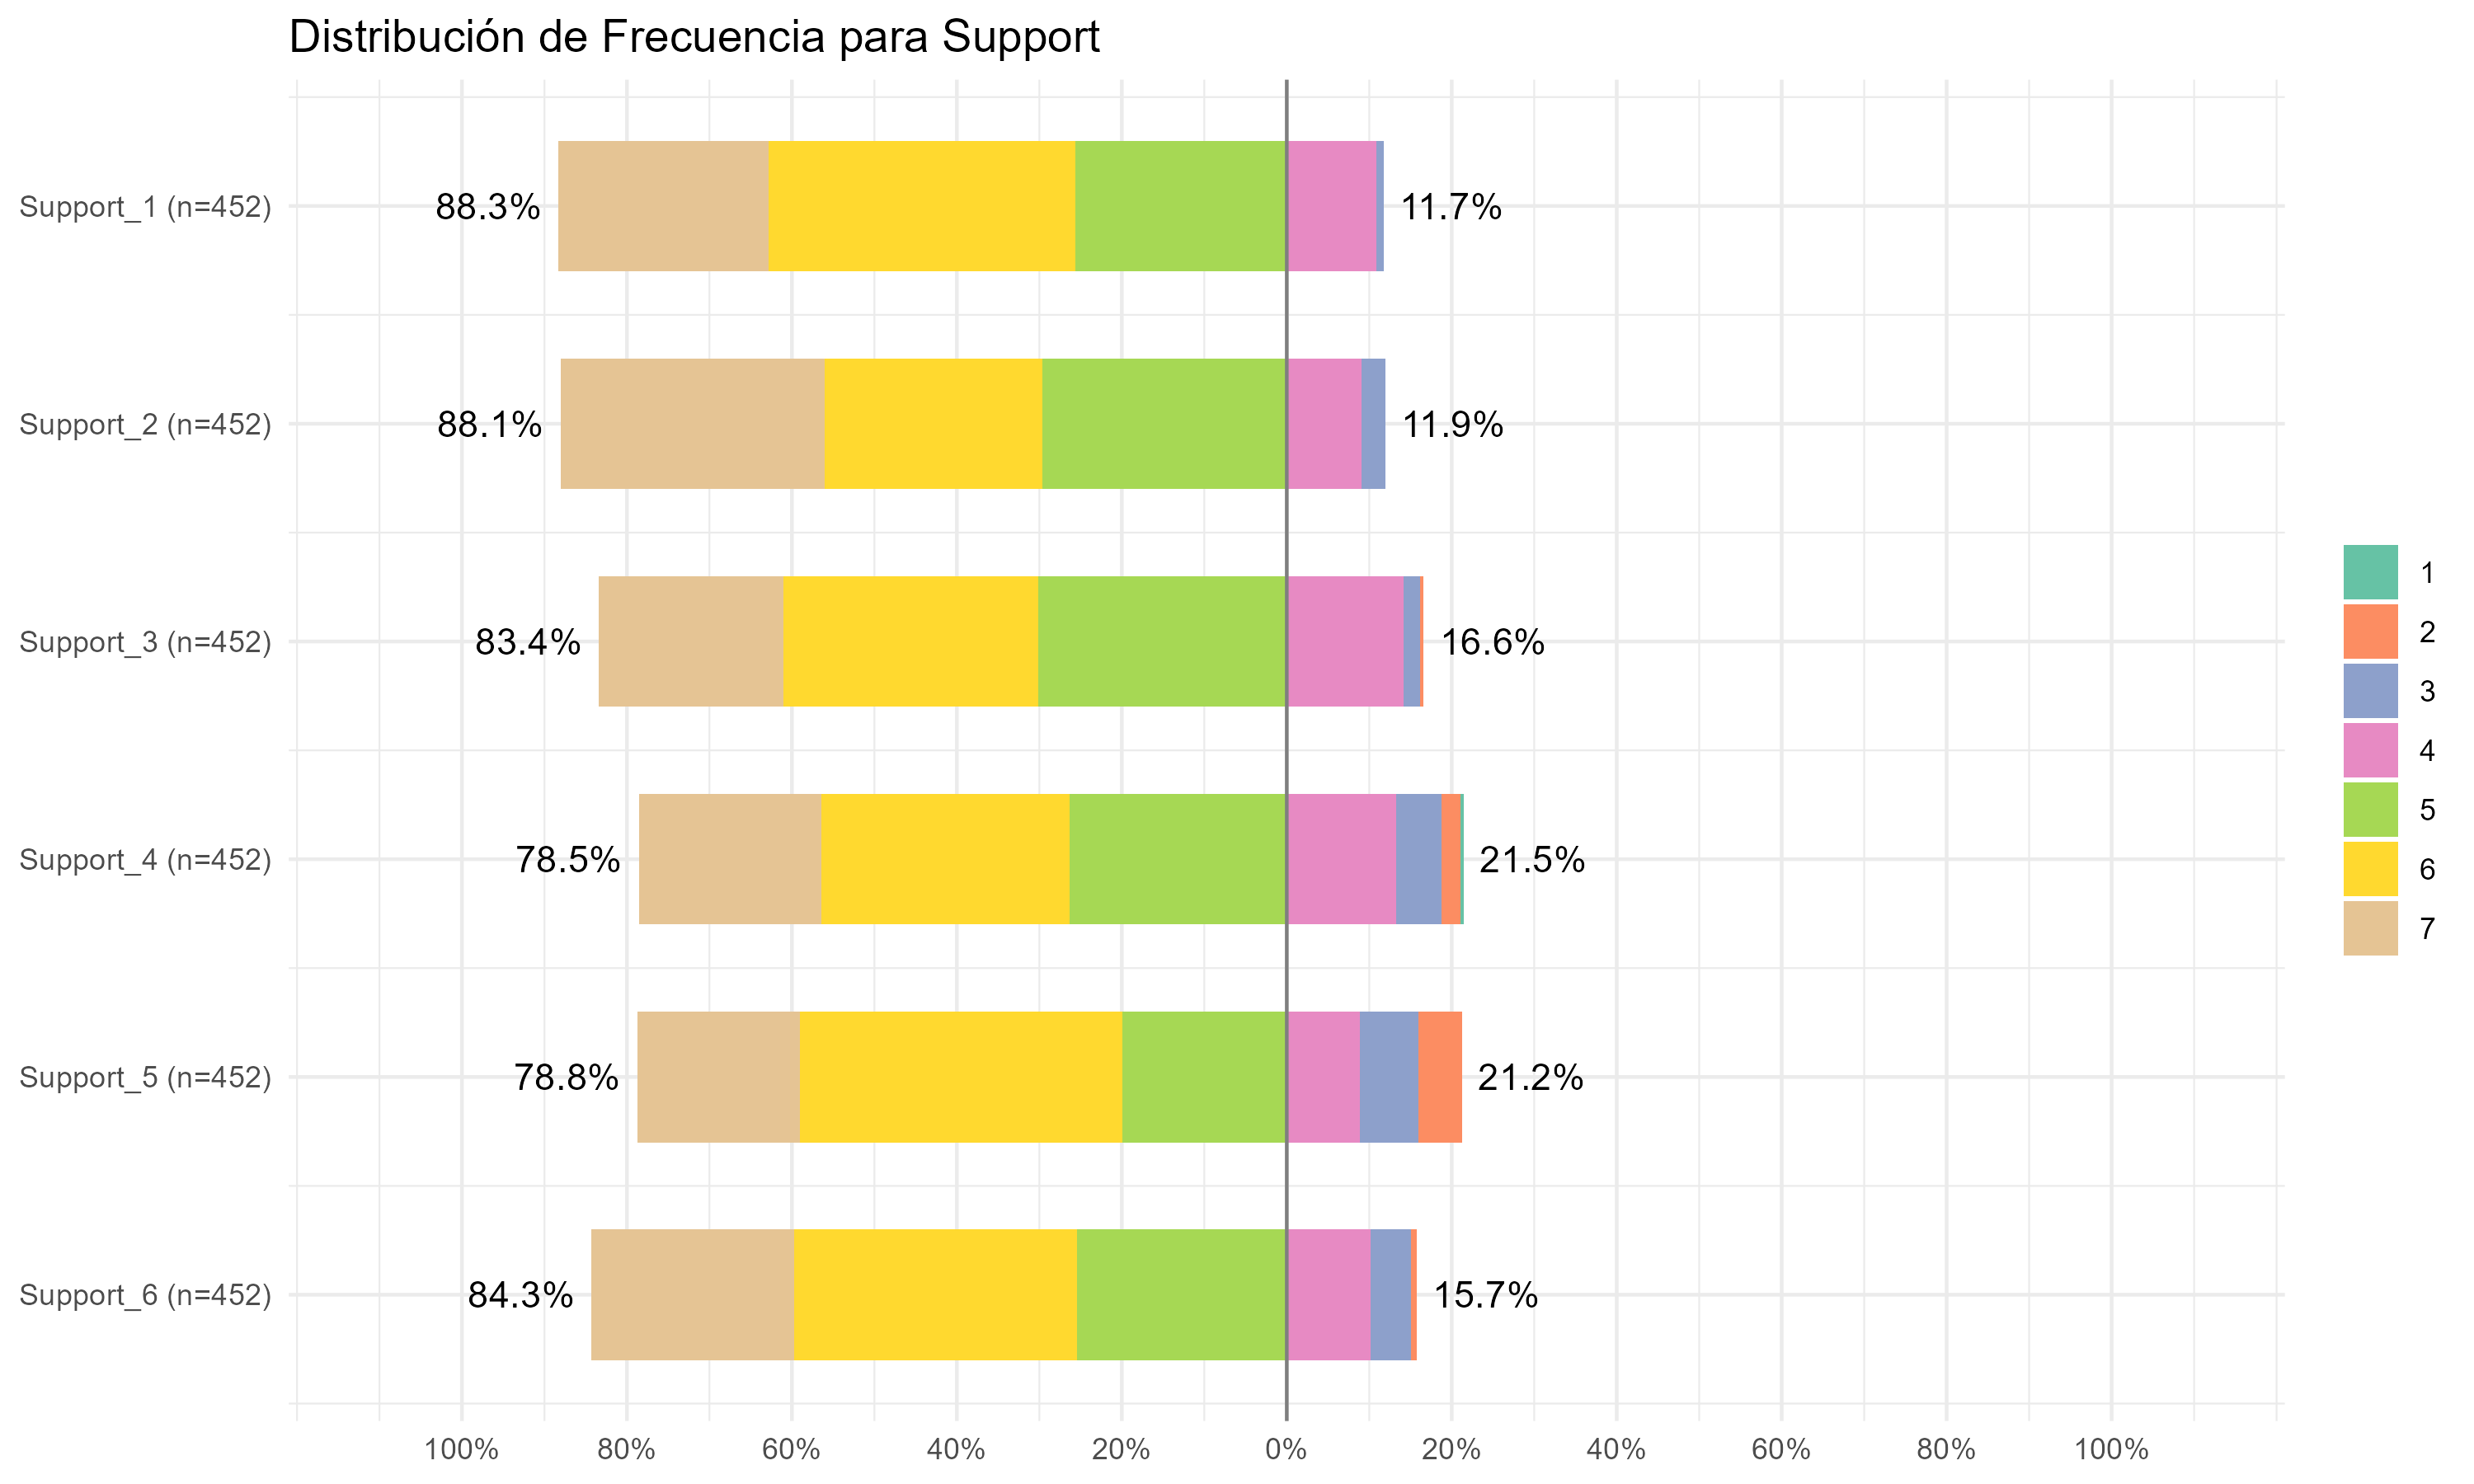
\includegraphics[width=0.45\textwidth]{figures/distribucion_frecuencia_Support.png} & 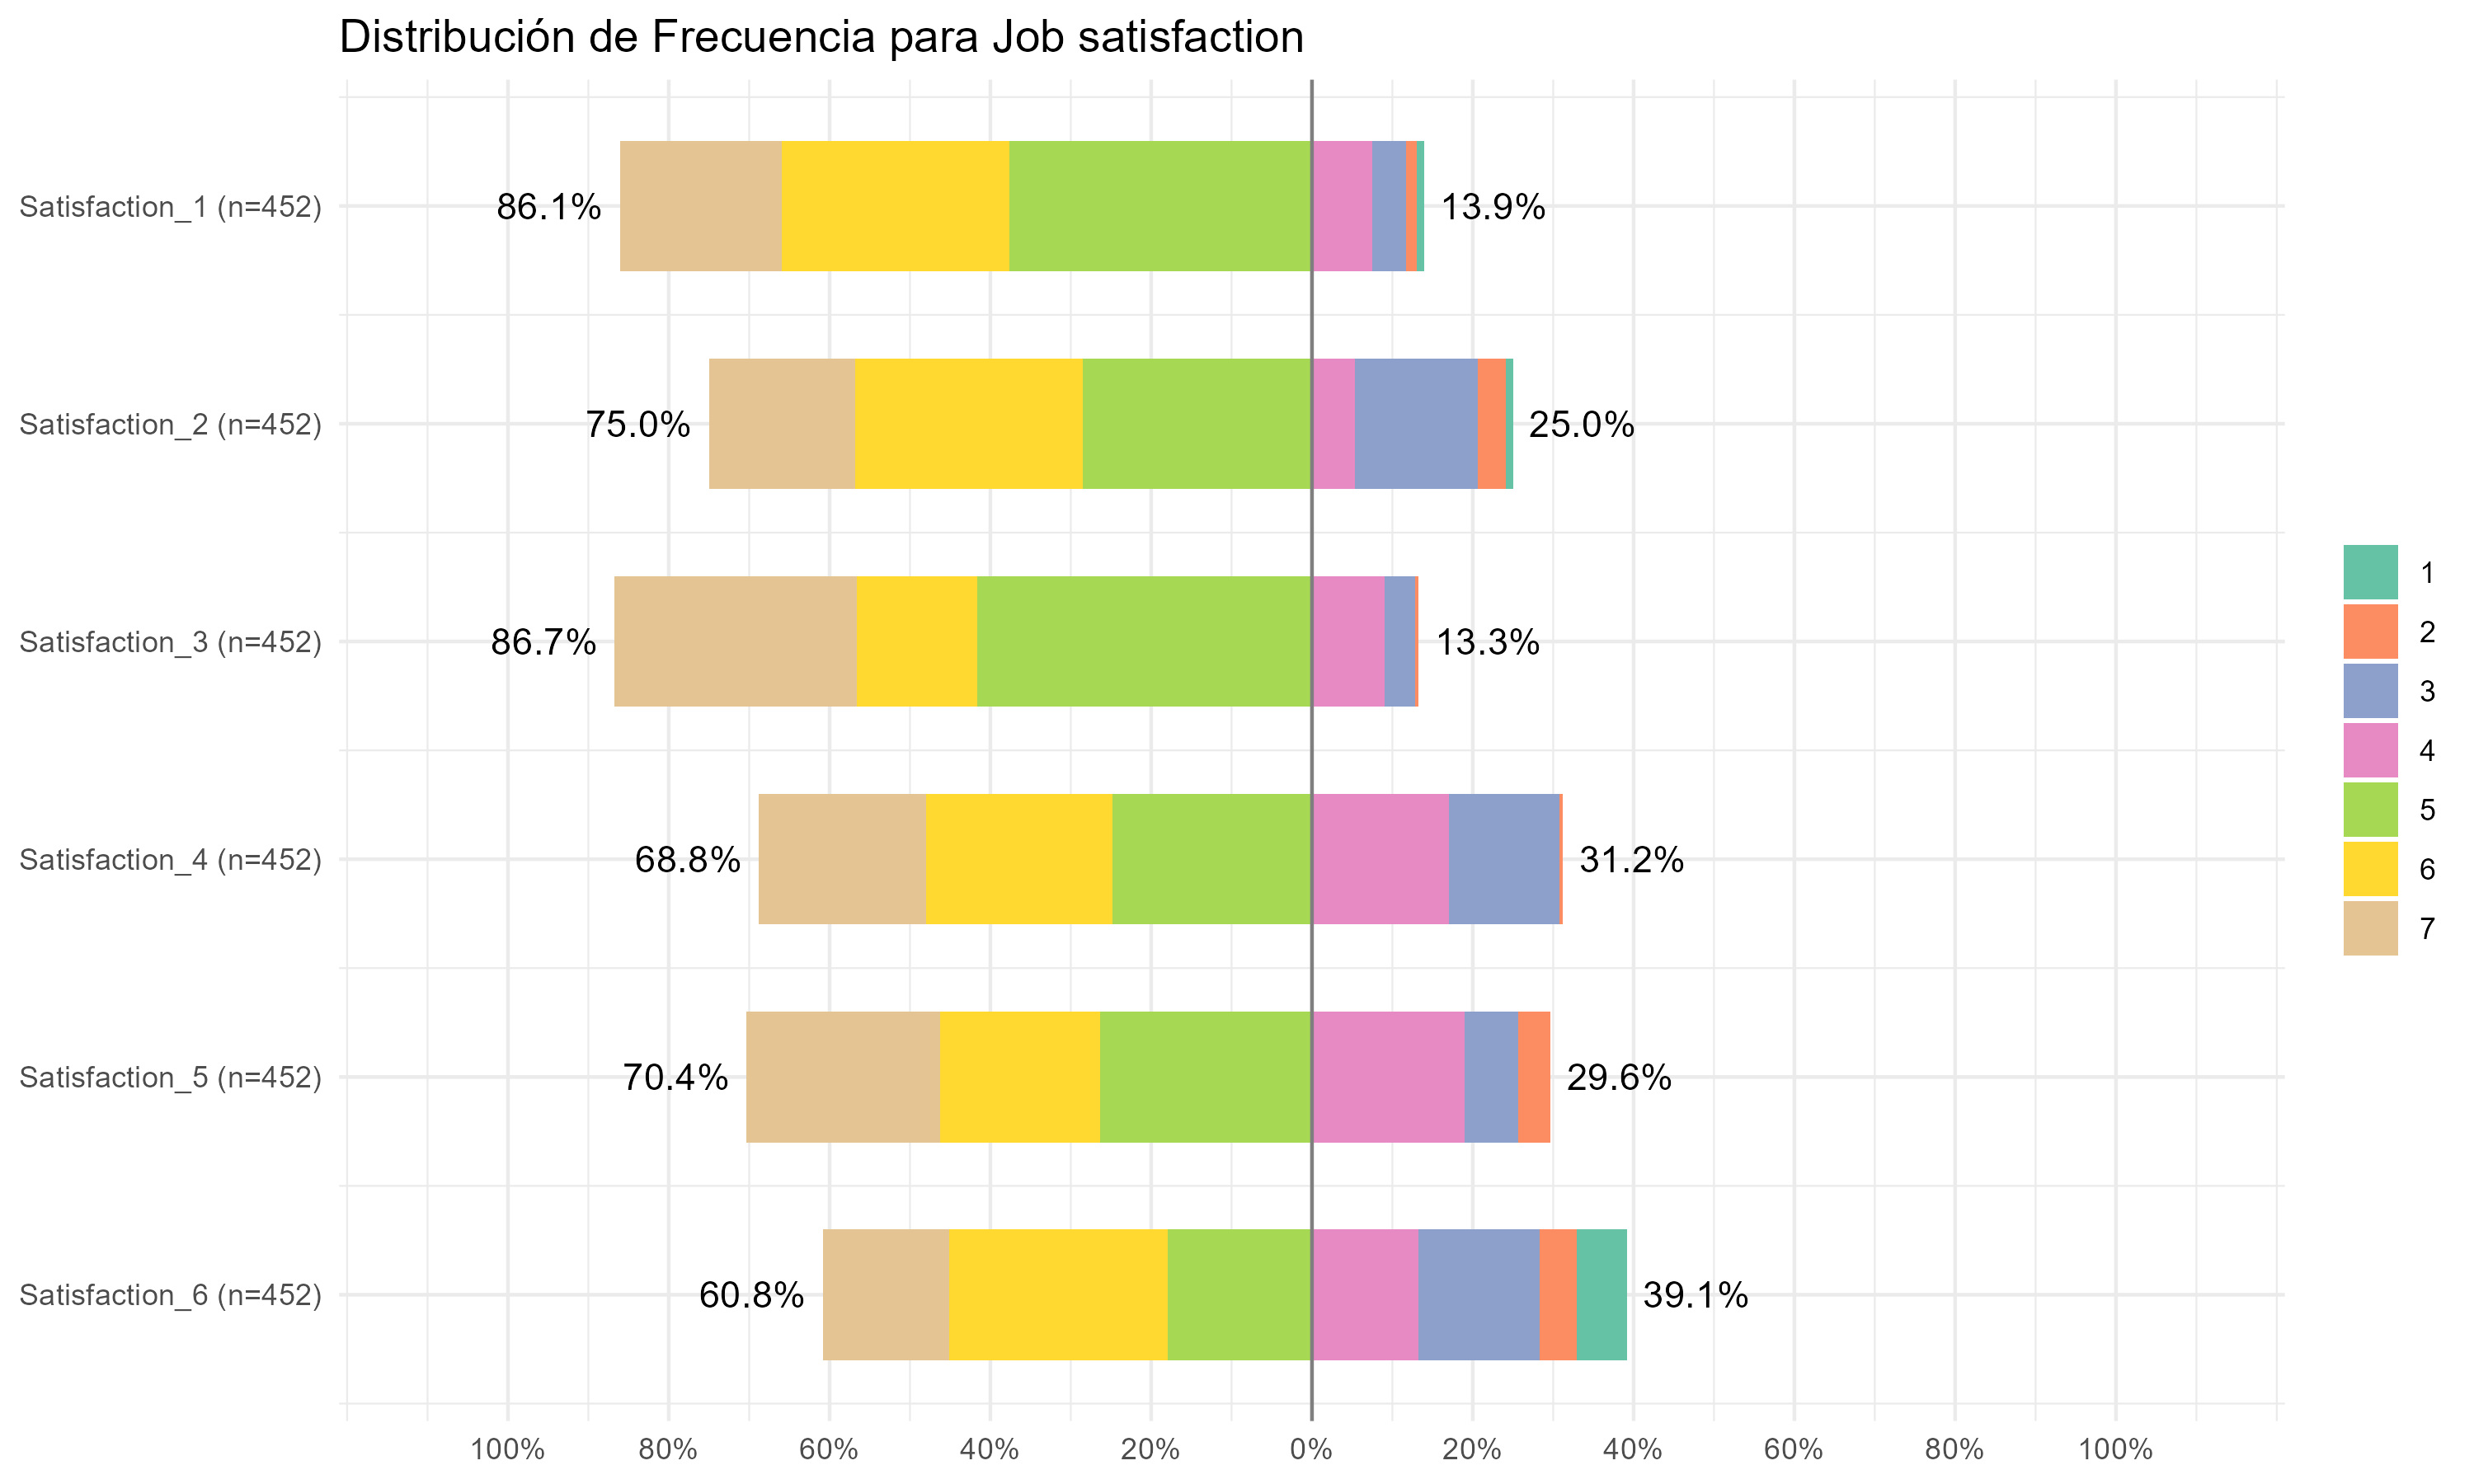
\includegraphics[width=0.45\textwidth]{figures/distribucion_frecuencia_satisfaction.png} \\
\multicolumn{2}{c}{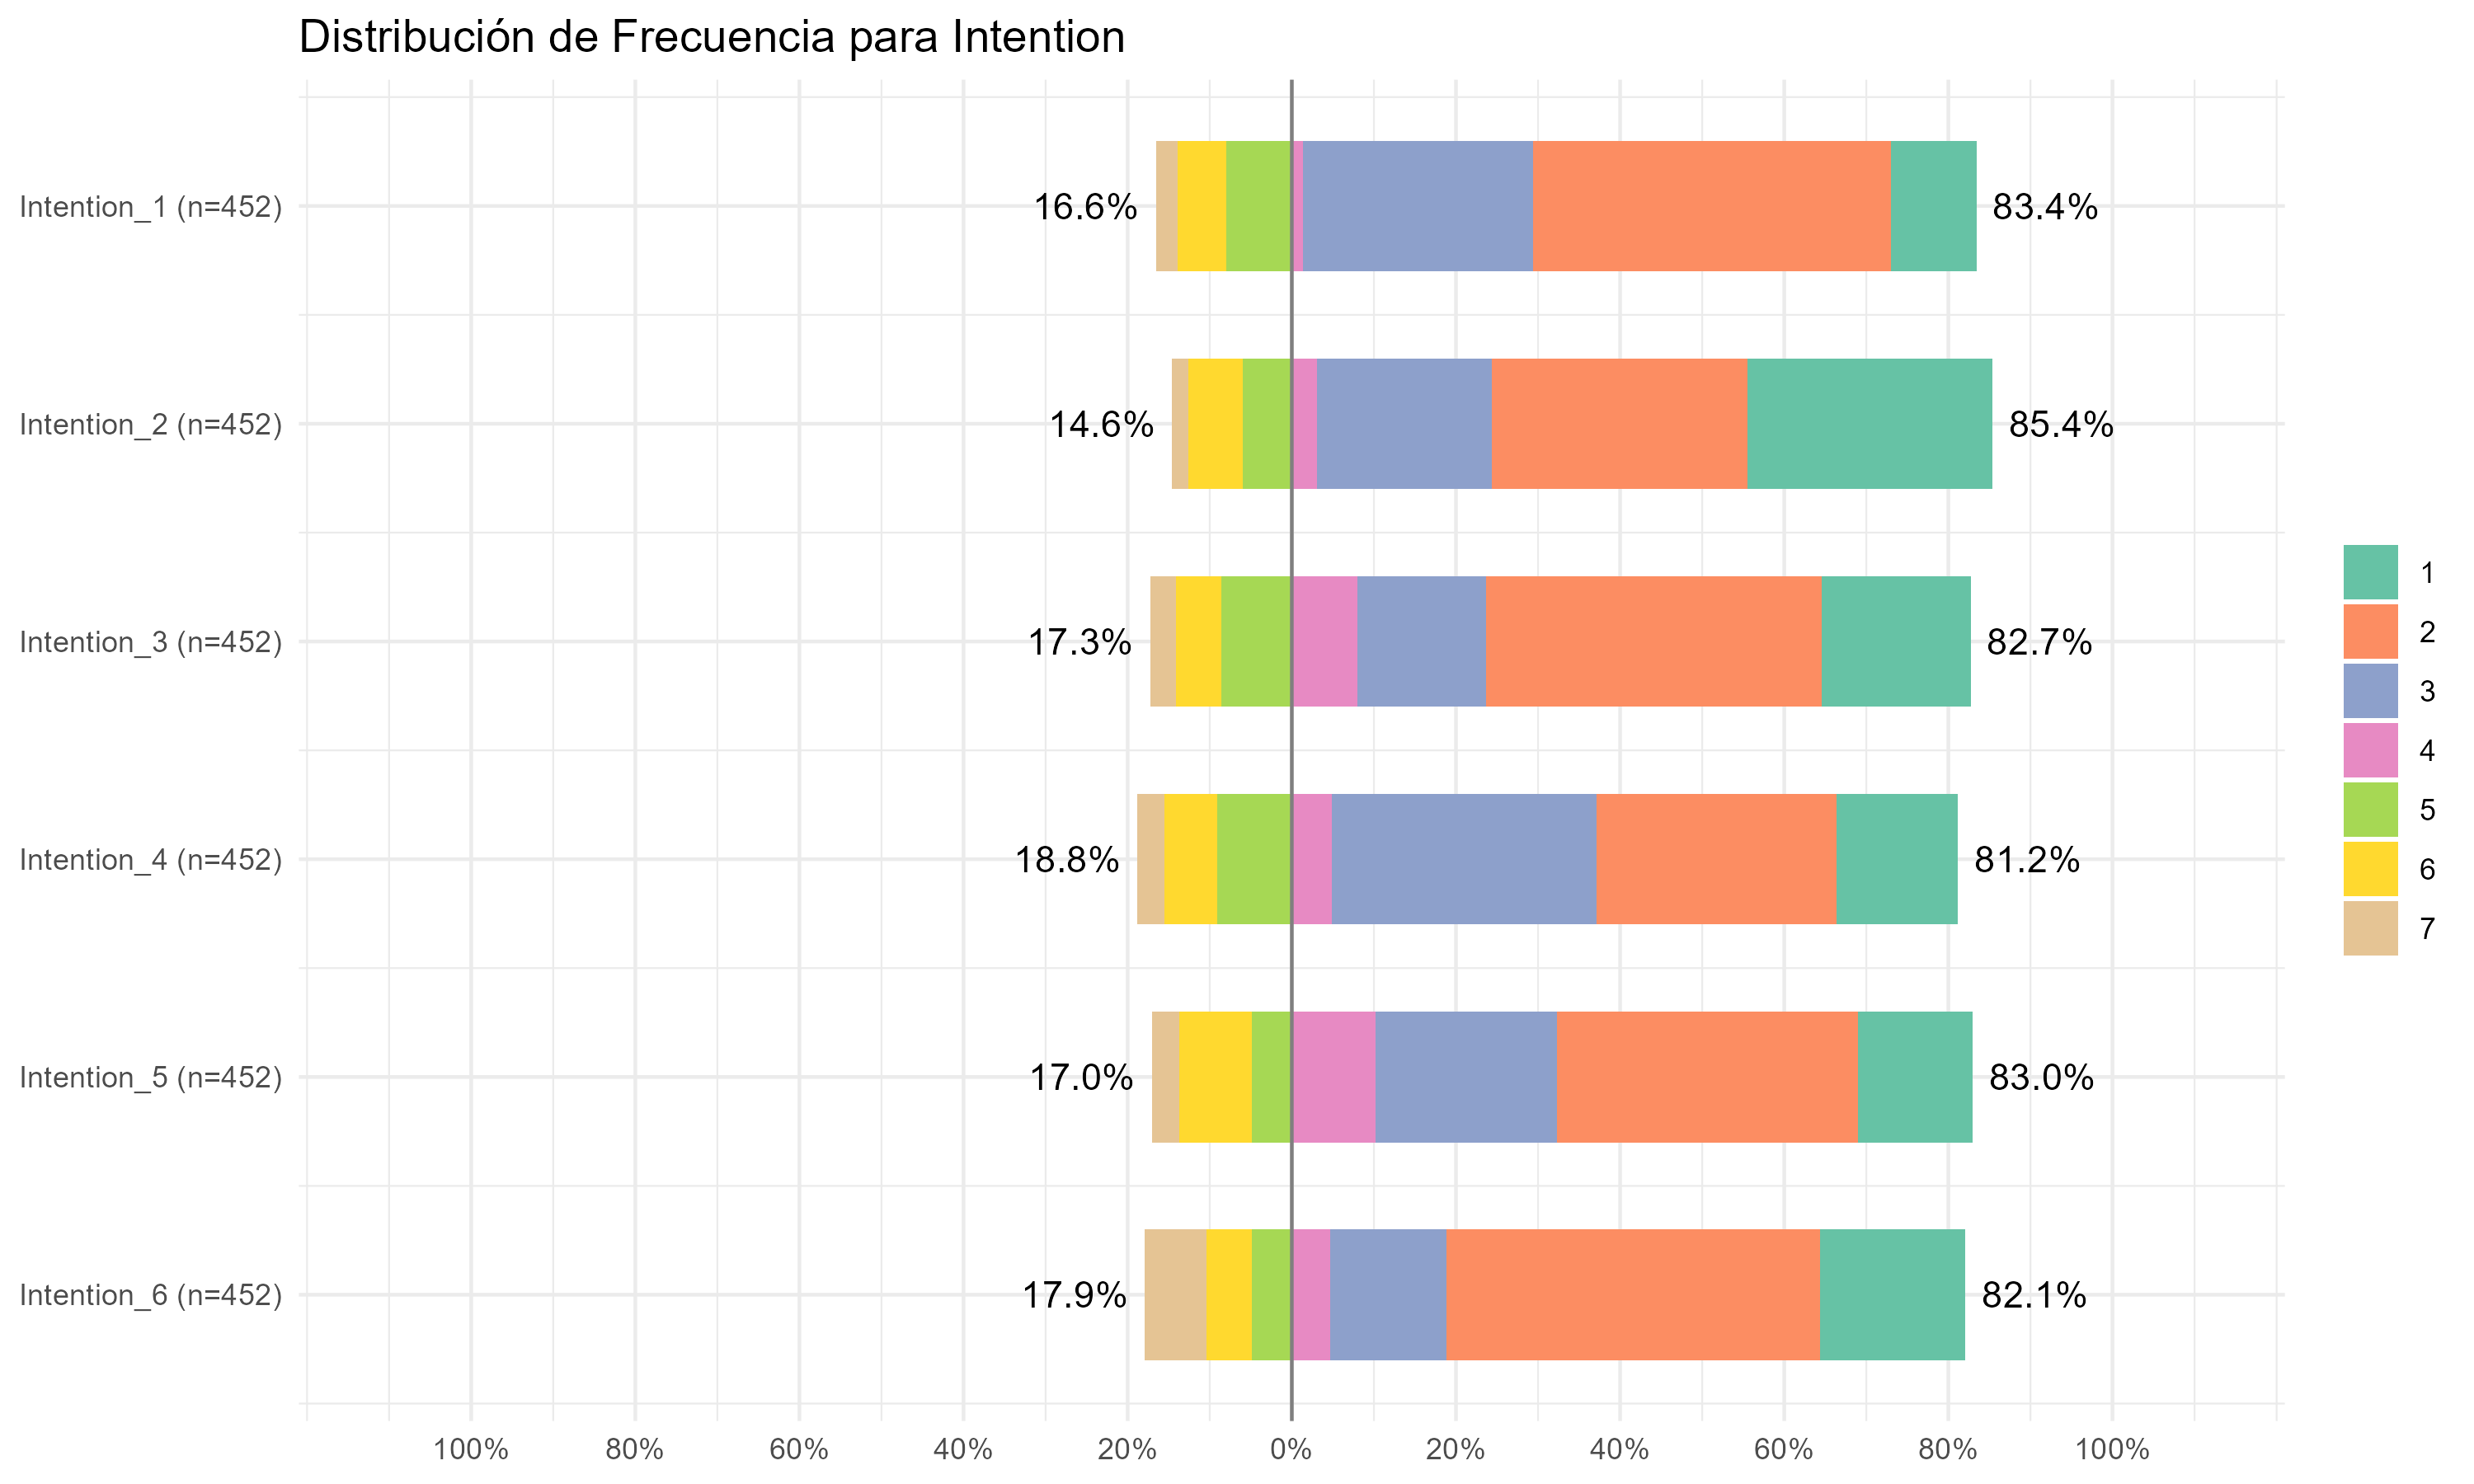
\includegraphics[width=0.45\textwidth]{figures/distribucion_frecuencia_Intention.png}}
\end{tabular}
\caption{Distribuciones de frecuencia de las cinco escalas Likert (1–7). De izquierda a derecha y de arriba hacia abajo: \emph{Skill--Job Fit}, \emph{Personality--Job Fit}, \emph{Apoyo Organizacional Percibido}, \emph{Satisfacción Laboral} e \emph{Intención de Renuncia}.}
\label{fig:histogramas}
\end{figure}

En términos de fiabilidad, la Tabla \ref{tab:fiabilidad} muestra los índices obtenidos mediante Teoría Clásica de los Tests (alfa de Cronbach, alfa ordinal, omega total y Límite Inferior de Guttman). Todas las escalas alcanzaron coeficientes alfa superiores a .87 y omegas mayores a .95, evidenciando buena consistencia interna y ausencia de ítems problemáticos. Las correlaciones ítem-total superaron .60 en la mayoría de los casos y los valores “alpha-if-item-deleted” no evidenciaron mejoras al eliminar ningún ítem, por lo que se conservaron las versiones completas de seis ítems por escala en esta etapa.

\begin{table}[htbp]
\centering
\caption{Índices de fiabilidad de las escalas (\(N=452\))}
\label{tab:fiabilidad}
\small
\begin{tabular}{@{}lccccc@{}}
\toprule
\textbf{Escala} & \textbf{Ítems} & \textbf{$\alpha$} & \textbf{$\alpha_{\text{ord}}$} & \textbf{$\omega$} & \textbf{GLB} \\
\midrule
Skill--Job Fit          & 6 & .917 & .940 & .959 & .959 \\
Personality--Job Fit    & 6 & .876 & .897 & .955 & .955 \\
Satisfacción Laboral    & 6 & .929 & .948 & .972 & .972 \\
Apoyo Organizacional    & 6 & .904 & .929 & .959 & .959 \\
Intención de Renuncia   & 6 & .962 & .959 & .971 & .971 \\
\bottomrule
\end{tabular}
\end{table}

\subsection{Estructura factorial: análisis exploratorio y confirmatorio}
Previo al AFC y al SEM se examinó la estructura subyacente mediante Análisis Factorial Exploratorio (AFE). La Tabla \ref{tab:kmo-bartlett-resumen} resume los resultados de la adecuación muestral (índice KMO) y la esfericidad (prueba de Bartlett) para cada subescala y para el instrumento completo. Todos los KMO superaron .80 (adecuación meritoria), con un KMO global = .90, y las pruebas de Bartlett fueron altamente significativas ($p<.001$), confirmando que la factorización es viable a nivel local y global.

\begin{table}[htbp]
\centering
\caption{Adecuación muestral y esfericidad por subescala (AFE, $n_{\text{AFE}}\approx150$)}
\label{tab:kmo-bartlett-resumen}
\small
\begin{tabular}{@{}lcccc@{}}
\toprule
\textbf{Subescala} & \textbf{KMO} & \textbf{$\chi^2$ de Bartlett} & \textbf{gl} & \textbf{$p$} \\
\midrule
Skill--Job Fit                & .90 &  665.53  &  15 & $<.001$ \\
Personality--Job Fit          & .80 &  574.20  &  15 & $<.001$ \\
Satisfacción Laboral          & .91 &  753.47  &  15 & $<.001$ \\
Intención de Renuncia         & .92 & 1088.89  &  15 & $<.001$ \\
Apoyo Organizacional (POS)    & .86 &  515.68  &  15 & $<.001$ \\
\midrule
\textbf{Instrumento completo} & .90 & 11188.96 & 435 & $<.001$ \\
\bottomrule
\end{tabular}
\end{table}

Para comprobar la unidimensionalidad de cada subescala se realizaron AFEs independientes forzando un factor por bloque (bloque = 6 ítems). La Tabla \ref{tab:unidimensionalidad-bloques} muestra el rango de cargas factoriales estandarizadas (\(\lambda\)), las comunalidades ($h^2$) y la varianza explicada por cada factor. Todas las subescalas presentaron cargas altas (rango .72–.96), comunalidades entre .52 y .93, varianza explicada $\geq .65$ y RMSR $<.12$, confirmando unidimensionalidad robusta.

\begin{table}[htbp]
\centering
\caption{Evidencia de unidimensionalidad por subescala (AFE; minres + oblimin, $n_{\text{AFE}}\approx150$)}
\label{tab:unidimensionalidad-bloques}
\small
\begin{tabular}{@{}lccccc@{}}
\toprule
\textbf{Subescala} & \textbf{Rango $\lambda$} & \textbf{Rango $h^2$} & \textbf{Var. expl.} & \textbf{RMSR} & \textbf{Interpretación} \\
\midrule
Skill--Job Fit           & .73--.94 & .54--.88 & .72 & .05–.07  & Unidimensional \\
Personality--Job Fit     & .72--.93 & .52--.87 & .65 & .09–.12  & Unidimensional \\
Satisfacción Laboral     & .81--.94 & .66--.88 & .78 & .03–.04  & Unidimensional \\
Intención de Renuncia    & .85--.96 & .73--.93 & .83 & .02–.03  & Unidimensional \\
Apoyo Organizacional     & .73--.87 & .53--.75 & .66 & .07–.09  & Unidimensional \\
\bottomrule
\end{tabular}
\end{table}

Para contrastar la estructura teórica de cinco factores, se estimaron dos AFE sobre los 30 ítems: un modelo unidimensional y otro de cinco factores oblicuos. El modelo de un solo factor mostró un ajuste pobre (RMSR = .16) y explicó sólo el 44 \% de la varianza común, por lo que se descartó la unidimensionalidad global. En cambio, el modelo de cinco factores presentó un RMSR de .04, explicó alrededor del 75 \% de la varianza común y reprodujo los dominios teóricos con correlaciones interfactoriales moderadas (0.18–0.51). La Tabla \ref{tab:efa-comparacion} resume esta comparación.

\begin{table}[htbp]
\centering
\caption{Comparación de modelos de AFE sobre los 30 ítems ($n_{\text{AFE}}\approx150$)}
\label{tab:efa-comparacion}
\small
\begin{tabular}{@{}lccc@{}}
\toprule
\textbf{Modelo} & \textbf{Var. expl.} & \textbf{RMSR} & \textbf{Interpretación} \\
\midrule
1 factor                & .44 & .16 & Ajuste pobre; descarta unidimensionalidad \\
5 factores oblicuos     & .75 & .04 & Ajuste excelente; estructura multifactorial \\
\bottomrule
\end{tabular}
\end{table}

El diagrama factorial exploratorio (Figura~\ref{fig:afe}) ilustra gráficamente la estructura de cinco factores obtenida con minres + oblimin, destacando las cargas estandarizadas de cada ítem y las correlaciones interfactoriales.

\begin{figure}[htbp]
\centering
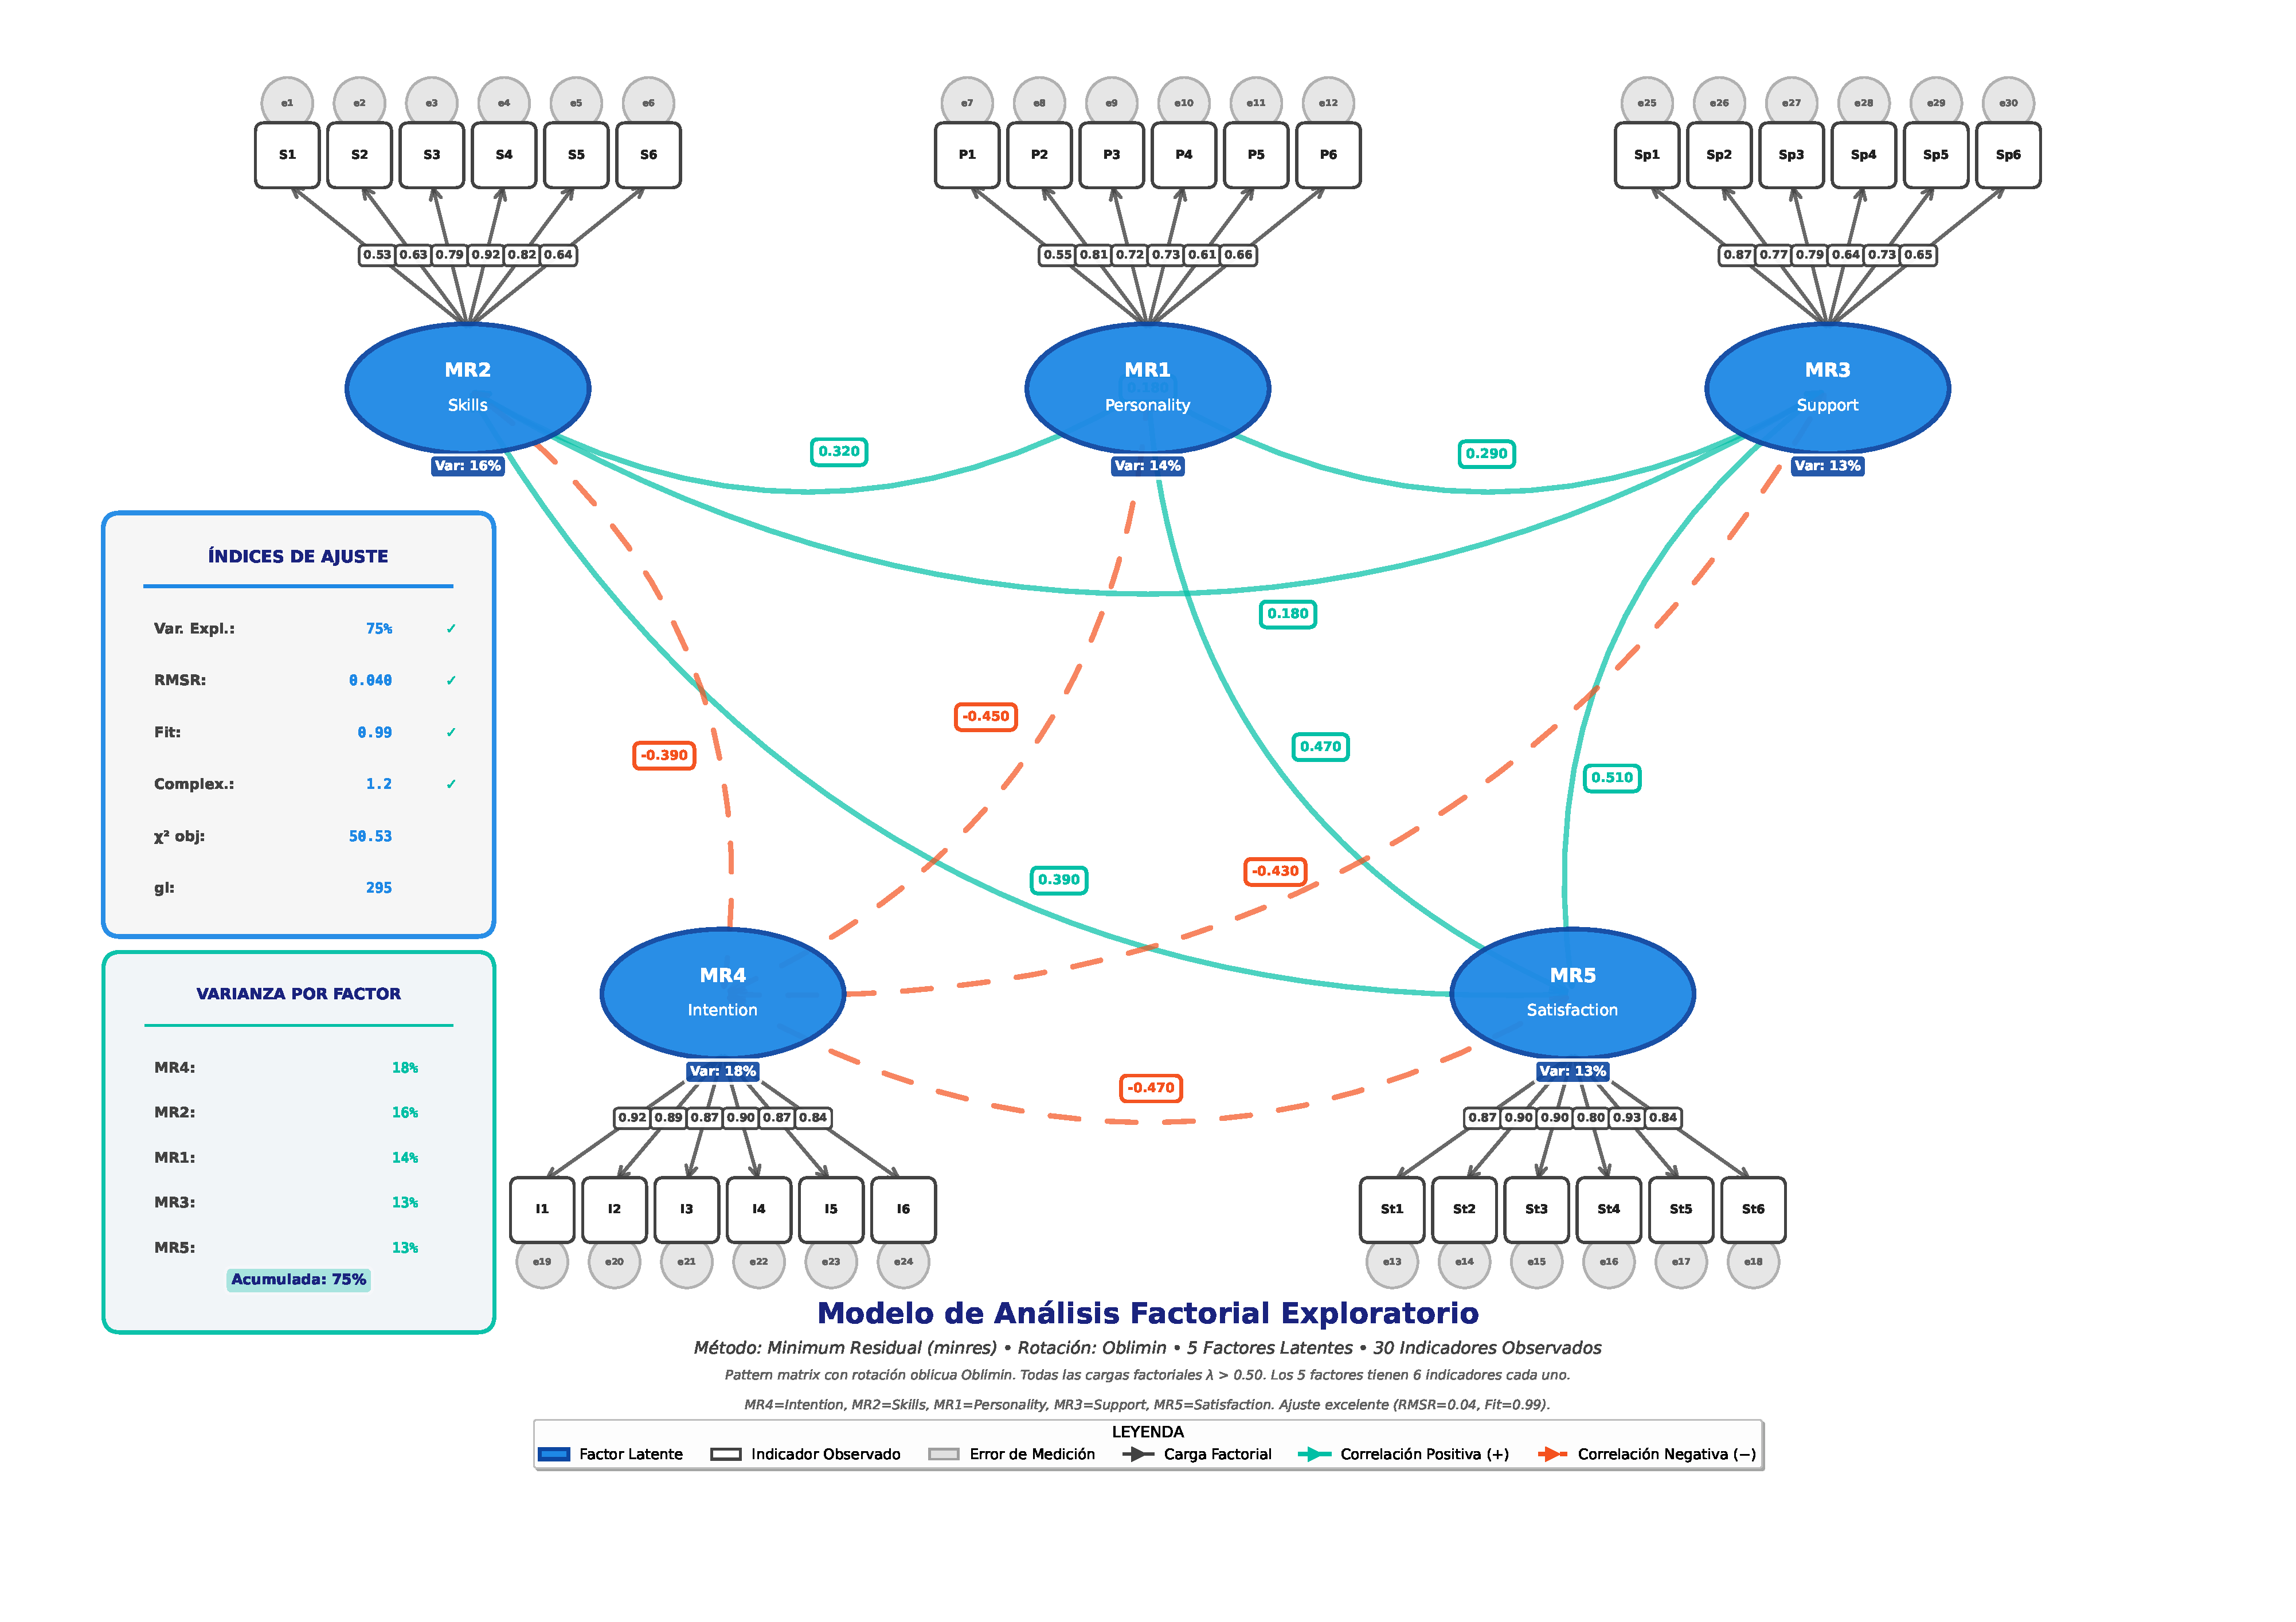
\includegraphics[width=0.9\textwidth]{figures/Diagrama_AFE_CORRECTO_FINAL.pdf}
\caption{Modelo factorial exploratorio de cinco factores (AFE; minres + oblimin, $n_{\text{AFE}}\approx150$). Se muestran las cargas estandarizadas por factor y las correlaciones interfactoriales.}
\label{fig:afe}
\end{figure}

\subsubsection*{Análisis factorial confirmatorio (AFC)}
La estructura de cinco factores se validó mediante AFC con estimador WLSMV sobre la submuestra de confirmación ($n_{\text{AFC}}\approx302$). El modelo presentó un ajuste global adecuado: $\chi^2/\mathrm{df} < 3$, $\mathrm{CFI}=.99$, $\mathrm{TLI}=.99$, $\mathrm{RMSEA}=.074$ [IC 90\,\% .068–.079] y $\mathrm{SRMR}=.063$. Todas las cargas estandarizadas fueron significativas ($p<.001$) y en su mayoría superiores a .70; los rangos fueron: \emph{Skill} (.66–.92), \emph{Personality} (.72–.89), \emph{Satisfaction} (.78–.93), \emph{Intention} (.80–.97) y \emph{POS} (.75–.97). La fiabilidad compuesta (CR) y la varianza media extraída (AVE) superaron .87 y .67, respectivamente, mientras que los índices HTMT estuvieron por debajo de .85, confirmando validez convergente y discriminante. La Figura \ref{fig:cfa} muestra el modelo confirmatorio estimado.

\begin{figure}[htbp]
\centering
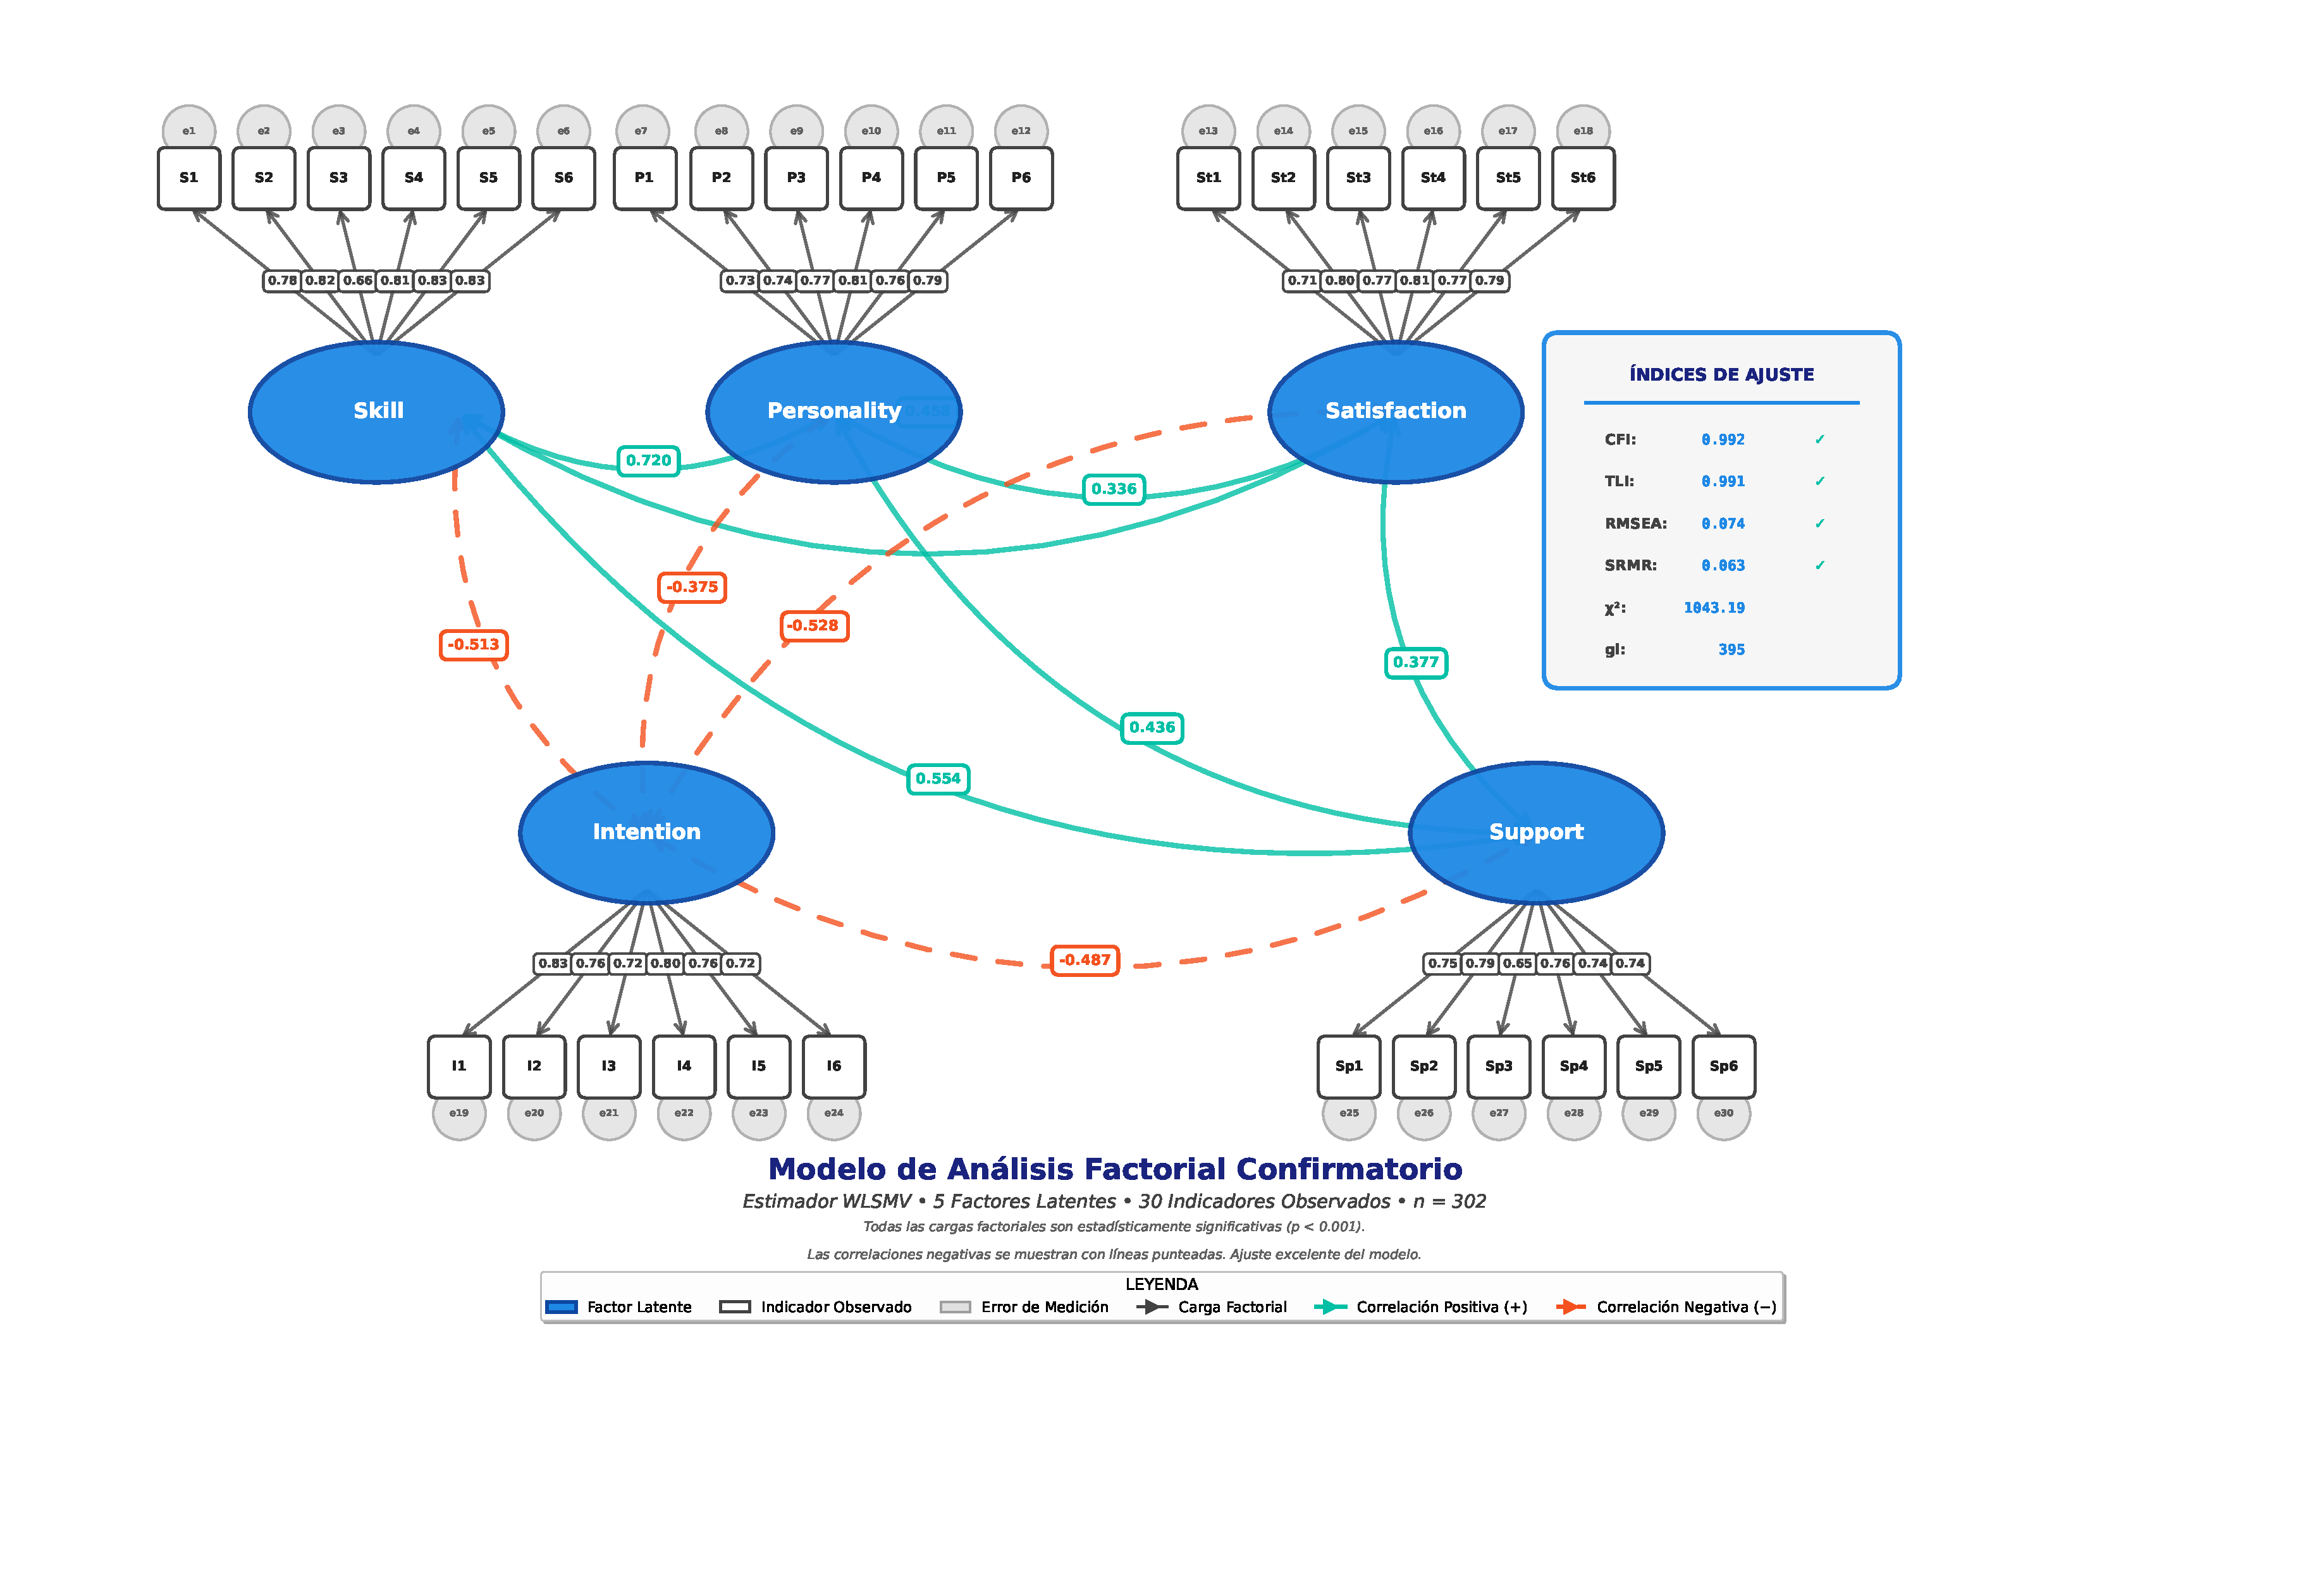
\includegraphics[width=0.9\textwidth]{figures/Diagrama_CFA_WLSMV_Ajustado_Final.pdf}
\caption{Modelo confirmatorio (AFC) estimado con WLSMV (5 factores, 30 indicadores, $n_{\text{AFC}}\approx302$).}
\label{fig:cfa}
\end{figure}

\subsection{Depuración de ítems mediante Teoría de Respuesta al Ítem (TRI)}
Aunque el modelo CFA completo mostró buen ajuste, sus índices no alcanzaron los criterios de excelencia (CFI/TLI $\approx.96$, RMSEA $\approx.075$). Se empleó el modelo de respuesta graduada de Samejima para seleccionar, por cada factor, los tres ítems con mayor discriminación y mejor ajuste, reduciendo el instrumento de 30 a 15 ítems. Los indicadores retenidos fueron: Skill\_2, Skill\_5, Skill\_6; Personality\_3, Personality\_4, Personality\_5; Satisfaction\_2, Satisfaction\_3, Satisfaction\_5; Support\_1, Support\_2, Support\_3; e Intention\_2, Intention\_3, Intention\_4. Este procedimiento preservó la representatividad de cada factor, mejoró la fiabilidad y simplificó la aplicación futura.

Para ilustrar el comportamiento de los ítems en el modelo GRM, la Figura \ref{fig:irt} muestra un ejemplo de curvas de información y curvas características de un ítem (curvas ICC) para una de las escalas. Se observa la alta capacidad discriminativa y los umbrales ordenados en las siete categorías.

\begin{figure}[htbp]
\centering
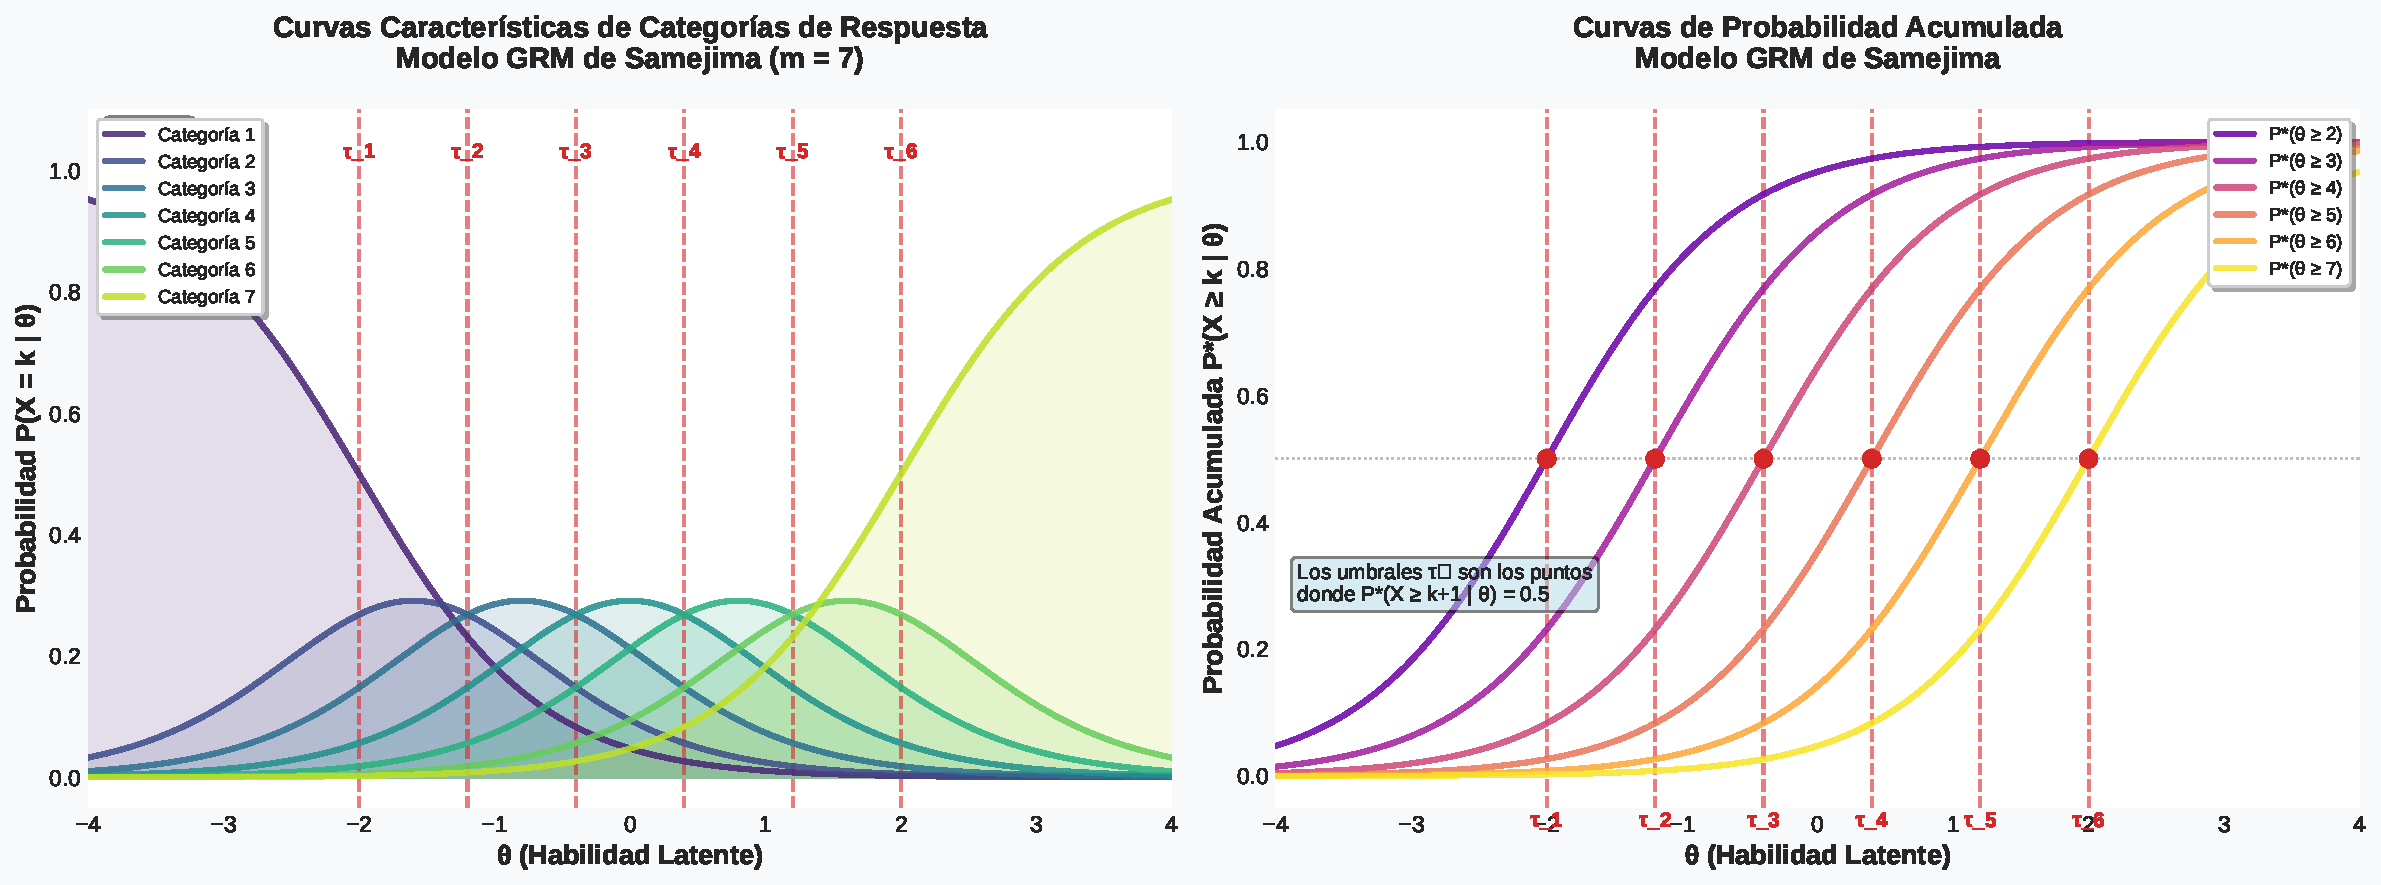
\includegraphics[width=0.8\textwidth]{figures/grm_samejima.pdf}
\caption{Curvas de información e ICC del modelo de respuesta graduada (TRI) para las escalas.}
\label{fig:irt}
\end{figure}

La depuración mediante TRI arrojó beneficios significativos: (a) incrementó la razón casos/parámetros de 6.0 a 10.0, mejorando la estabilidad numérica; (b) elevó los índices de ajuste del SEM (CFI=0.994; TLI=0.993; RMSEA=0.049; SRMR=0.040); (c) concentró la información en ítems óptimos (cargas promedio $\lambda=.87$) y eliminó redundancias; y (d) redujo la carga de respuesta para futuros estudios.

\subsection{Modelo estructural}
\subsubsection*{Modelo completo (30 ítems)}
Validado el modelo de medición, se ajustó el SEM completo con 30 indicadores para evaluar las hipótesis H1–H7. El modelo alcanzó un ajuste aceptable: CFI$_{\text{scaled}}=.963$, TLI$_{\text{scaled}}=.960$, RMSEA$_{\text{scaled}}=.075$ y SRMR=.067. La Figura \ref{fig:sem-completo} presenta el diagrama estructural.

\begin{figure}[htbp]
\centering
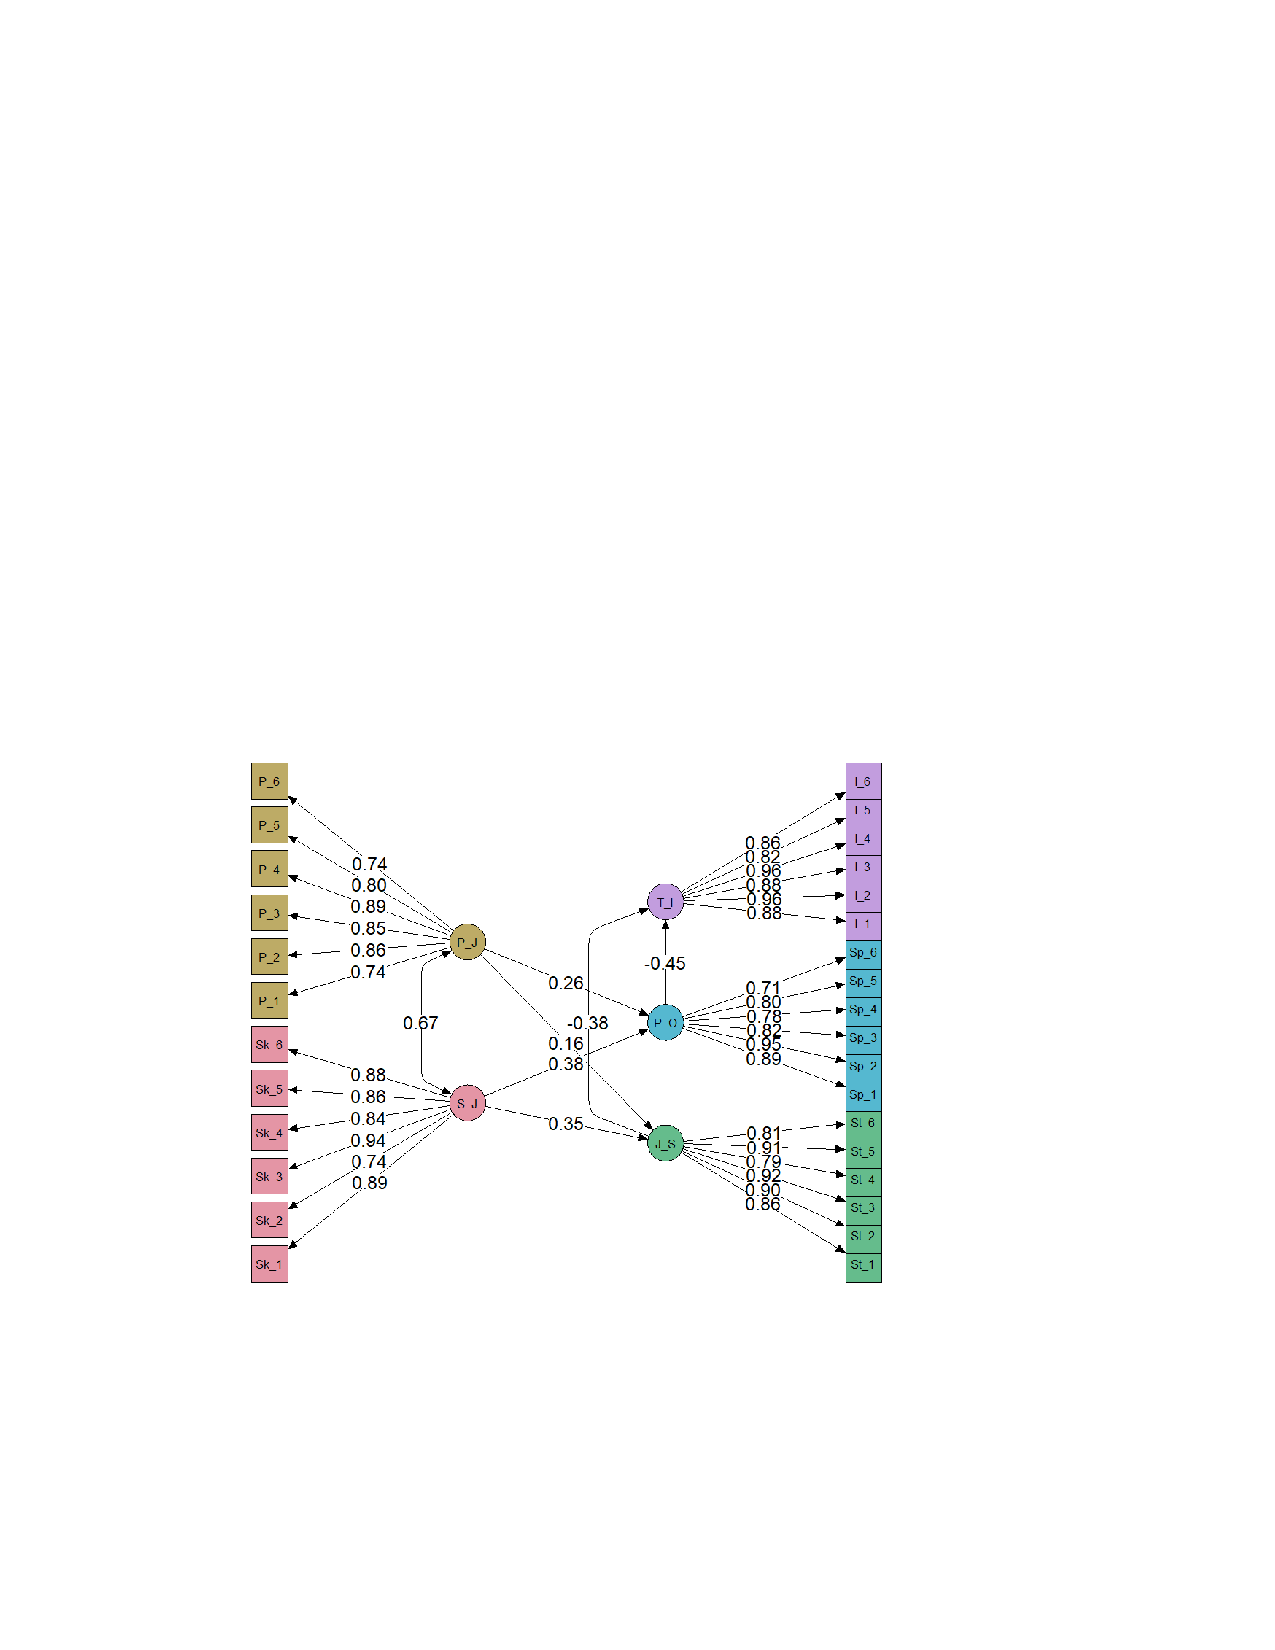
\includegraphics[width=0.9\textwidth]{figures/modelo0.pdf}
\caption{Modelo de ecuaciones estructurales completo con 30 indicadores observables (5 factores correlacionados).}
\label{fig:sem-completo}
\end{figure}

Los coeficientes directos estandarizados (Tabla \ref{tab:sem-completo-paths}) mostraron que el \emph{Skill--Job Fit} predice positivamente la satisfacción ($\beta=.347$) y el POS ($\beta=.377$), mientras que el \emph{Personality--Job Fit} predice la satisfacción de forma más moderada ($\beta=.156$) y el POS ($\beta=.264$). A su vez, la satisfacción ($\beta=-.385$) y el POS ($\beta=-.449$) se asociaron negativamente con la intención de renuncia, explicando un 44.4\,\% de su varianza. Los efectos indirectos indicaron mediaciones significativas de Skill y Personality a través de satisfacción y POS (Tabla \ref{tab:sem-completo-indirect}). Todas las hipótesis (H1–H7) fueron respaldadas.

\begin{table}[htbp]
\centering
\caption{Coeficientes directos estandarizados del SEM completo (30 ítems, $N=452$)}
\label{tab:sem-completo-paths}
\small
\begin{tabular}{@{}lccc@{}}
\toprule
\textbf{Ruta} & \textbf{$\beta$} & \textbf{SE} & \textbf{$p$} \\
\midrule
Satisfacción $\leftarrow$ Skill                 & .347 & .063 & $<.001$ \\
Satisfacción $\leftarrow$ Personality           & .156 & .063 & $<.001$ \\
POS $\leftarrow$ Skill                          & .377 & .070 & $<.001$ \\
POS $\leftarrow$ Personality                    & .264 & .067 & $<.001$ \\
Intention $\leftarrow$ Satisfacción             & $-.385$ & .053 & $<.001$ \\
Intention $\leftarrow$ POS                      & $-.449$ & .048 & $<.001$ \\
\multicolumn{4}{l}{\textit{Varianza explicada}} \\
\quad $R^2$(Satisfacción)  & \multicolumn{3}{l}{.217 (21.7\,\%)} \\
\quad $R^2$(POS)           & \multicolumn{3}{l}{.345 (34.5\,\%)} \\
\quad $R^2$(Intention)     & \multicolumn{3}{l}{.444 (44.4\,\%)} \\
\bottomrule
\end{tabular}
\end{table}

\begin{table}[htbp]
\centering
\caption{Efectos indirectos (mediaciones) en el SEM completo}
\label{tab:sem-completo-indirect}
\small
\begin{tabular}{@{}lccc@{}}
\toprule
\textbf{Ruta indirecta} & \textbf{$\beta_{\text{ind}}$} & \textbf{SE} & \textbf{$p$} \\
\midrule
Skill → Satisfacción → Intention          & $-.134$ & .037 & $<.001$ \\
Skill → POS → Intention                    & $-.169$ & .041 & $<.001$ \\
\multicolumn{2}{l}{Skill → Intention (indirecto total)} & \multicolumn{2}{l}{$-.303$} \\
Personality → Satisfacción → Intention    & $-.060$ & .028 & .033 \\
Personality → POS → Intention             & $-.118$ & .036 & $<.001$ \\
\multicolumn{2}{l}{Personality → Intention (indirecto total)} & \multicolumn{2}{l}{$-.179$} \\
\bottomrule
\end{tabular}
\end{table}

\subsubsection*{Modelo parsimonioso (15 ítems)}
Tras la depuración por TRI, el SEM se reestimó con los 15 indicadores seleccionados. El ajuste del modelo parsimonioso fue excelente: CFI$_{\text{scaled}}=.994$, TLI$_{\text{scaled}}=.993$, RMSEA$_{\text{scaled}}=.049$ [IC 90\,\% .038–.059] y SRMR=.040. La Figura \ref{fig:sem-parsimonioso} muestra el diagrama del SEM reducido.

\begin{figure}[htbp]
\centering
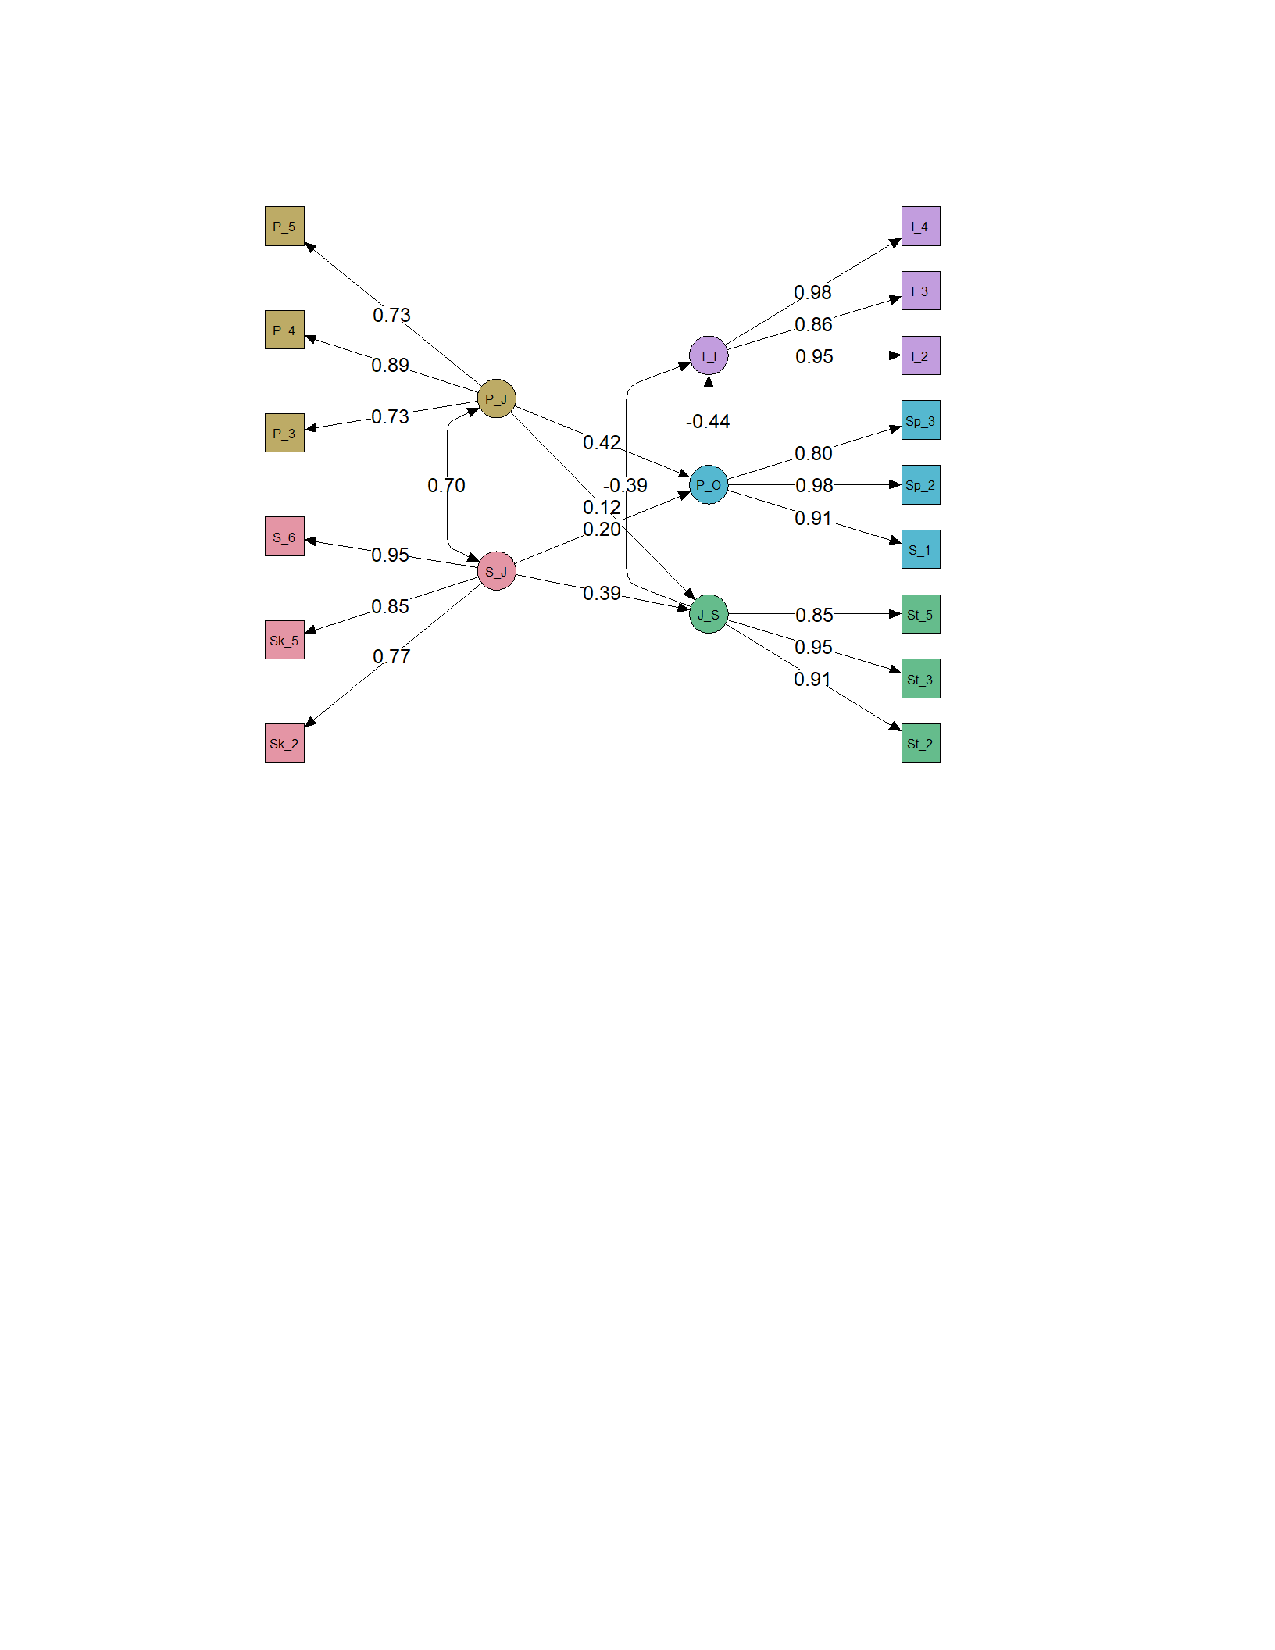
\includegraphics[width=0.9\textwidth]{figures/modelosem_216.pdf}
\caption{Modelo de ecuaciones estructurales parsimonioso con 15 indicadores seleccionados mediante TRI.}
\label{fig:sem-parsimonioso}
\end{figure}

Los coeficientes directos en el modelo parsimonioso se mantuvieron en la misma dirección y con magnitudes muy similares al modelo completo, aunque ligeramente superiores. En particular, el \emph{Skill--Job Fit} continuó siendo un predictor robusto de satisfacción y POS; el \emph{Personality--Job Fit} mostró efectos significativos en el POS pero no en la satisfacción; y tanto la satisfacción como el POS siguieron reduciendo la intención de renuncia de forma significativa. La varianza explicada aumentó ligeramente: $R^2$(Satisfacción)=.267, $R^2$(POS)=.373, $R^2$(Intention)=.459. La comparación entre ambos modelos se resume en la Tabla \ref{tab:comparacion-modelos}.

\begin{table}[htbp]
\centering
\caption{Comparación de índices de ajuste: modelos completo vs. parsimonioso}
\label{tab:comparacion-modelos}
\small
\begin{tabular}{@{}lcccc@{}}
\toprule
\textbf{Índice} & \textbf{Modelo completo} & \textbf{Modelo parsimonioso} & \textbf{$\Delta$} & \textbf{Mejora} \\
\midrule
$\chi^2$ (gl)               & 1403.43 (398)  & 171.21 (83)    & $-1232.22$ & Sí \\
CFI$_{\text{scaled}}$       & .963           & .994          & +.031     & Sí \\
TLI$_{\text{scaled}}$       & .960           & .993          & +.033     & Sí \\
RMSEA$_{\text{scaled}}$     & .075 [.071,.079] & .049 [.038,.059] & $-.026$ & Sí \\
SRMR                        & .067           & .040          & $-.027$ & Sí \\
\# de parámetros libres     & 75             & 45            & $-30$   & +Parsimonia \\
Razón casos/parámetro       & 6.0            & 10.0          & +4.0    & +Estabilidad \\
\bottomrule
\end{tabular}
\end{table}

\subsubsection*{Resumen de hallazgos}
En síntesis, los resultados empíricos revelan que:

\begin{itemize}
\item Las cinco escalas mostraron distribuciones sesgadas hacia valores altos (excepto Intention) y una excelente fiabilidad interna. La correlación ítem-total y los índices de fiabilidad (alfa, omega, GLB) confirmaron que ningún ítem requería ser eliminado inicialmente.
\item El AFE evidenció una estructura de cinco factores claramente diferenciados, con altas cargas y comunalidades, así como KMO meritorios y Bartlett significativos. El modelo unidimensional fue descartado por su pobre ajuste.
\item El AFC confirmó la estructura de cinco factores con cargas estandarizadas altas y fiabilidad compuesta y AVE superiores a .87 y .67 respectivamente; la validez discriminante quedó respaldada mediante el criterio de Fornell–Larcker y los índices HTMT.
\item La depuración mediante TRI permitió reducir el instrumento a 15 ítems (tres por factor) conservando la estructura conceptual. El modelo SEM parsimonioso con 15 indicadores mostró un ajuste excelente (CFI/TLI $> .99$, RMSEA $< .05$, SRMR $< .05$) y mejoró la razón casos/parámetro, demostrando que un instrumento breve puede captar la misma estructura y producir estimaciones más estables.
\item En ambos modelos SEM, el ajuste técnico (\emph{Skill--Job Fit}) tuvo un impacto mayor que el ajuste socio-cultural (\emph{Personality--Job Fit}) en la satisfacción laboral y en el apoyo organizacional percibido. El POS fue el predictor más fuerte de la reducción de la intención de renuncia, seguido de la satisfacción. Las mediaciones a través de POS y satisfacción fueron significativas, con un efecto indirecto total de Skill sobre Intention de \(-.303\) (modelo completo) y \(-.413\) (modelo parsimonioso).
\item Estos hallazgos respaldan las siete hipótesis planteadas (H1–H7), confirman la relevancia del ajuste persona–trabajo y del apoyo organizacional percibido como mecanismos que reducen la intención de renuncia en tecnólogos colombianos, y demuestran que una versión abreviada del instrumento ofrece ventajas de parsimonia y precisión sin sacrificar validez ni fiabilidad.
\end{itemize}


